\documentclass{ximera}
%%% Begin Laad packages

\makeatletter
\@ifclassloaded{xourse}{%
    \typeout{Start loading preamble.tex (in a XOURSE)}%
    \def\isXourse{true}   % automatically defined; pre 112022 it had to be set 'manually' in a xourse
}{%
    \typeout{Start loading preamble.tex (NOT in a XOURSE)}%
}
\makeatother

\def\isEn\true 

\pgfplotsset{compat=1.16}

\usepackage{currfile}

% 201908/202301: PAS OP: babel en doclicense lijken problemen te veroorzaken in .jax bestand
% (wegens syntax error met toegevoegde \newcommands ...)
\pdfOnly{
    \usepackage[type={CC},modifier={by-nc-sa},version={4.0}]{doclicense}
    %\usepackage[hyperxmp=false,type={CC},modifier={by-nc-sa},version={4.0}]{doclicense}
    %%% \usepackage[dutch]{babel}
}



\usepackage[utf8]{inputenc}
\usepackage{morewrites}   % nav zomercursus (answer...?)
\usepackage{multirow}
\usepackage{multicol}
\usepackage{tikzsymbols}
\usepackage{ifthen}
%\usepackage{animate} BREAKS HTML STRUCTURE USED BY XIMERA
\usepackage{relsize}

\usepackage{eurosym}    % \euro  (€ werkt niet in xake ...?)
\usepackage{fontawesome} % smileys etc

% Nuttig als ook interactieve beamer slides worden voorzien:
\providecommand{\p}{} % default nothing ; potentially usefull for slides: redefine as \pause
%providecommand{\p}{\pause}

    % Layout-parameters voor het onderschrift bij figuren
\usepackage[margin=10pt,font=small,labelfont=bf, labelsep=endash,format=hang]{caption}
%\usepackage{caption} % captionof
%\usepackage{pdflscape}    % landscape environment

% Met "\newcommand\showtodonotes{}" kan je todonotes tonen (in pdf/online)
% 201908: online werkt het niet (goed)
\providecommand\showtodonotes{disable}
\providecommand\todo[1]{\typeout{TODO #1}}
%\usepackage[\showtodonotes]{todonotes}
%\usepackage{todonotes}

%
% Poging tot aanpassen layout
%
\usepackage{tcolorbox}
\tcbuselibrary{theorems}

%%% Einde laad packages

%%% Begin Ximera specifieke zaken

\graphicspath{
	{../../}
	{../}
	{./}
  	{../../pictures/}
   	{../pictures/}
   	{./pictures/}
	{./explog/}    % M05 in groeimodellen       
}

%%% Einde Ximera specifieke zaken

%
% define softer blue/red/green, use KU Leuven base colors for blue (and dark orange for red ?)
%
% todo: rather redefine blue/red/green ...?
%\definecolor{xmblue}{rgb}{0.01, 0.31, 0.59}
%\definecolor{xmred}{rgb}{0.89, 0.02, 0.17}
\definecolor{xmdarkblue}{rgb}{0.122, 0.671, 0.835}   % KU Leuven Blauw
\definecolor{xmblue}{rgb}{0.114, 0.553, 0.69}        % KU Leuven Blauw
\definecolor{xmgreen}{rgb}{0.13, 0.55, 0.13}         % No KULeuven variant for green found ...

\definecolor{xmaccent}{rgb}{0.867, 0.541, 0.18}      % KU Leuven Accent (orange ...)
\definecolor{kuaccent}{rgb}{0.867, 0.541, 0.18}      % KU Leuven Accent (orange ...)

\colorlet{xmred}{xmaccent!50!black}                  % Darker version of KU Leuven Accent

\providecommand{\blue}[1]{{\color{blue}#1}}    
\providecommand{\red}[1]{{\color{red}#1}}

\renewcommand\CancelColor{\color{xmaccent!50!black}}

% werkt in math en text mode om MATH met oranje (of grijze...)  achtergond te tonen (ook \important{\text{blabla}} lijkt te werken)
%\newcommand{\important}[1]{\ensuremath{\colorbox{xmaccent!50!white}{$#1$}}}   % werkt niet in Mathjax
%\newcommand{\important}[1]{\ensuremath{\colorbox{lightgray}{$#1$}}}
\newcommand{\important}[1]{\ensuremath{\colorbox{orange}{$#1$}}}   % TODO: kleur aanpassen voor mathjax; wordt overschreven infra!


% Uitzonderlijk kan met \pdfnl in de PDF een newline worden geforceerd, die online niet nodig/nuttig is omdat daar de regellengte hoe dan ook niet gekend is.
\ifdefined\HCode%
\providecommand{\pdfnl}{}%
\else%
\providecommand{\pdfnl}{%
  \\%
}%
\fi

% Uitzonderlijk kan met \handoutnl in de handout-PDF een newline worden geforceerd, die noch online noch in de PDF-met-antwoorden nuttig is.
\ifdefined\HCode
\providecommand{\handoutnl}{}
\else
\providecommand{\handoutnl}{%
\ifhandout%
  \nl%
\fi%
}
\fi



% \cellcolor IGNORED by tex4ht ?
% \begin{center} seems not to wordk
    % (missing margin-left: auto;   on tabular-inside-center ???)
%\newcommand{\importantcell}[1]{\ensuremath{\cellcolor{lightgray}#1}}  %  in tabular; usablility to be checked
\providecommand{\importantcell}[1]{\ensuremath{#1}}     % no mathjax2 support for colloring array cells

\pdfOnly{
  \renewcommand{\important}[1]{\ensuremath{\colorbox{kuaccent!50!white}{$#1$}}}
  \renewcommand{\importantcell}[1]{\ensuremath{\cellcolor{kuaccent!40!white}#1}}   
}

%%% Tikz styles


\pgfplotsset{compat=1.16}

\usetikzlibrary{trees,positioning,arrows,fit,shapes,math,calc,decorations.markings,through,intersections,patterns,matrix}

\usetikzlibrary{decorations.pathreplacing,backgrounds}    % 5/2023: from experimental


\usetikzlibrary{angles,quotes}

\usepgfplotslibrary{fillbetween} % bepaalde_integraal
\usepgfplotslibrary{polar}    % oa voor poolcoordinaten.tex

\pgfplotsset{ownstyle/.style={axis lines = center, axis equal image, xlabel = $x$, ylabel = $y$, enlargelimits}} 

\pgfplotsset{
	plot/.style={no marks,samples=50}
}

\newcommand{\xmPlotsColor}{
	\pgfplotsset{
		plot1/.style={darkgray,no marks,samples=100},
		plot2/.style={lightgray,no marks,samples=100},
		plotresult/.style={blue,no marks,samples=100},
		plotblue/.style={blue,no marks,samples=100},
		plotred/.style={red,no marks,samples=100},
		plotgreen/.style={green,no marks,samples=100},
		plotpurple/.style={purple,no marks,samples=100}
	}
}
\newcommand{\xmPlotsBlackWhite}{
	\pgfplotsset{
		plot1/.style={black,loosely dashed,no marks,samples=100},
		plot2/.style={black,loosely dotted,no marks,samples=100},
		plotresult/.style={black,no marks,samples=100},
		plotblue/.style={black,no marks,samples=100},
		plotred/.style={black,dotted,no marks,samples=100},
		plotgreen/.style={black,dashed,no marks,samples=100},
		plotpurple/.style={black,dashdotted,no marks,samples=100}
	}
}


\newcommand{\xmPlotsColorAndStyle}{
	\pgfplotsset{
		plot1/.style={darkgray,no marks,samples=100},
		plot2/.style={lightgray,no marks,samples=100},
		plotresult/.style={blue,no marks,samples=100},
		plotblue/.style={xmblue,no marks,samples=100},
		plotred/.style={xmred,dashed,thick,no marks,samples=100},
		plotgreen/.style={xmgreen,dotted,very thick,no marks,samples=100},
		plotpurple/.style={purple,no marks,samples=100}
	}
}


%\iftikzexport
\xmPlotsColorAndStyle
%\else
%\xmPlotsBlackWhite
%\fi
%%%


%
% Om venndiagrammen te arceren ...
%
\makeatletter
\pgfdeclarepatternformonly[\hatchdistance,\hatchthickness]{north east hatch}% name
{\pgfqpoint{-1pt}{-1pt}}% below left
{\pgfqpoint{\hatchdistance}{\hatchdistance}}% above right
{\pgfpoint{\hatchdistance-1pt}{\hatchdistance-1pt}}%
{
	\pgfsetcolor{\tikz@pattern@color}
	\pgfsetlinewidth{\hatchthickness}
	\pgfpathmoveto{\pgfqpoint{0pt}{0pt}}
	\pgfpathlineto{\pgfqpoint{\hatchdistance}{\hatchdistance}}
	\pgfusepath{stroke}
}
\pgfdeclarepatternformonly[\hatchdistance,\hatchthickness]{north west hatch}% name
{\pgfqpoint{-\hatchthickness}{-\hatchthickness}}% below left
{\pgfqpoint{\hatchdistance+\hatchthickness}{\hatchdistance+\hatchthickness}}% above right
{\pgfpoint{\hatchdistance}{\hatchdistance}}%
{
	\pgfsetcolor{\tikz@pattern@color}
	\pgfsetlinewidth{\hatchthickness}
	\pgfpathmoveto{\pgfqpoint{\hatchdistance+\hatchthickness}{-\hatchthickness}}
	\pgfpathlineto{\pgfqpoint{-\hatchthickness}{\hatchdistance+\hatchthickness}}
	\pgfusepath{stroke}
}
%\makeatother

\tikzset{
    hatch distance/.store in=\hatchdistance,
    hatch distance=10pt,
    hatch thickness/.store in=\hatchthickness,
   	hatch thickness=2pt
}

\colorlet{circle edge}{black}
\colorlet{circle area}{blue!20}


\tikzset{
    filled/.style={fill=green!30, draw=circle edge, thick},
    arceerl/.style={pattern=north east hatch, pattern color=blue!50, draw=circle edge},
    arceerr/.style={pattern=north west hatch, pattern color=yellow!50, draw=circle edge},
    outline/.style={draw=circle edge, thick}
}




%%% Updaten commando's
\def\hoofding #1#2#3{\maketitle}     % OBSOLETE ??

% we willen (bijna) altijd \geqslant ipv \geq ...!
\newcommand{\geqnoslant}{\geq}
\renewcommand{\geq}{\geqslant}
\newcommand{\leqnoslant}{\leq}
\renewcommand{\leq}{\leqslant}

% Todo: (201908) waarom komt er (soms) underlined voor emph ...?
\renewcommand{\emph}[1]{\textit{#1}}

% API commando's

\newcommand{\ds}{\displaystyle}
\newcommand{\ts}{\textstyle}  % tegenhanger van \ds   (Ximera zet PER  DEFAULT \ds!)

% uit Zomercursus-macro's: 
\newcommand{\bron}[1]{\begin{scriptsize} \emph{#1} \end{scriptsize}}     % deprecated ...?


%definities nieuwe commando's - afkortingen veel gebruikte symbolen
\newcommand{\R}{\ensuremath{\mathbb{R}}}
\newcommand{\Rnul}{\ensuremath{\mathbb{R}_0}}
\newcommand{\Reen}{\ensuremath{\mathbb{R}\setminus\{1\}}}
\newcommand{\Rnuleen}{\ensuremath{\mathbb{R}\setminus\{0,1\}}}
\newcommand{\Rplus}{\ensuremath{\mathbb{R}^+}}
\newcommand{\Rmin}{\ensuremath{\mathbb{R}^-}}
\newcommand{\Rnulplus}{\ensuremath{\mathbb{R}_0^+}}
\newcommand{\Rnulmin}{\ensuremath{\mathbb{R}_0^-}}
\newcommand{\Rnuleenplus}{\ensuremath{\mathbb{R}^+\setminus\{0,1\}}}
\newcommand{\N}{\ensuremath{\mathbb{N}}}
\newcommand{\Nnul}{\ensuremath{\mathbb{N}_0}}
\newcommand{\Z}{\ensuremath{\mathbb{Z}}}
\newcommand{\Znul}{\ensuremath{\mathbb{Z}_0}}
\newcommand{\Zplus}{\ensuremath{\mathbb{Z}^+}}
\newcommand{\Zmin}{\ensuremath{\mathbb{Z}^-}}
\newcommand{\Znulplus}{\ensuremath{\mathbb{Z}_0^+}}
\newcommand{\Znulmin}{\ensuremath{\mathbb{Z}_0^-}}
\newcommand{\C}{\ensuremath{\mathbb{C}}}
\newcommand{\Cnul}{\ensuremath{\mathbb{C}_0}}
\newcommand{\Cplus}{\ensuremath{\mathbb{C}^+}}
\newcommand{\Cmin}{\ensuremath{\mathbb{C}^-}}
\newcommand{\Cnulplus}{\ensuremath{\mathbb{C}_0^+}}
\newcommand{\Cnulmin}{\ensuremath{\mathbb{C}_0^-}}
\newcommand{\Q}{\ensuremath{\mathbb{Q}}}
\newcommand{\Qnul}{\ensuremath{\mathbb{Q}_0}}
\newcommand{\Qplus}{\ensuremath{\mathbb{Q}^+}}
\newcommand{\Qmin}{\ensuremath{\mathbb{Q}^-}}
\newcommand{\Qnulplus}{\ensuremath{\mathbb{Q}_0^+}}
\newcommand{\Qnulmin}{\ensuremath{\mathbb{Q}_0^-}}

\newcommand{\perdef}{\overset{\mathrm{def}}{=}}
\newcommand{\pernot}{\overset{\mathrm{notatie}}{=}}
\newcommand\perinderdaad{\overset{!}{=}}     % voorlopig gebruikt in limietenrekenregels
\newcommand\perhaps{\overset{?}{=}}          % voorlopig gebruikt in limietenrekenregels

\newcommand{\degree}{^\circ}


\DeclareMathOperator{\dom}{dom}     % domein
\DeclareMathOperator{\codom}{codom} % codomein
\DeclareMathOperator{\bld}{bld}     % beeld
\DeclareMathOperator{\graf}{graf}   % grafiek
\DeclareMathOperator{\rico}{rico}   % richtingcoëfficient
\DeclareMathOperator{\co}{co}       % coordinaat
\DeclareMathOperator{\gr}{gr}       % graad

\newcommand{\func}[5]{\ensuremath{#1: #2 \rightarrow #3: #4 \mapsto #5}} % Easy to write a function


% Operators
\DeclareMathOperator{\bgsin}{bgsin}
\DeclareMathOperator{\bgcos}{bgcos}
\DeclareMathOperator{\bgtan}{bgtan}
\DeclareMathOperator{\bgcot}{bgcot}
\DeclareMathOperator{\bgsinh}{bgsinh}
\DeclareMathOperator{\bgcosh}{bgcosh}
\DeclareMathOperator{\bgtanh}{bgtanh}
\DeclareMathOperator{\bgcoth}{bgcoth}

% Oude \Bgsin etc deprecated: gebruik \bgsin, en herdefinieer dat als je Bgsin wil!
%\DeclareMathOperator{\cosec}{cosec}    % not used? gebruik \csc en herdefinieer

% operatoren voor differentialen: to be verified; 1/2020: inconsequent gebruik bij afgeleiden/integralen
\renewcommand{\d}{\mathrm{d}}
\newcommand{\dx}{\d x}
\newcommand{\dd}[1]{\frac{\mathrm{d}}{\mathrm{d}#1}}
\newcommand{\ddx}{\dd{x}}

% om in voorbeelden/oefeningen de notatie voor afgeleiden te kunnen kiezen
% Usage: \afg{(2\sin(x))}  (en wordt d/dx, of accent, of D )
%\newcommand{\afg}[1]{{#1}'}
\newcommand{\afg}[1]{\left(#1\right)'}
%\renewcommand{\afg}[1]{\frac{\mathrm{d}#1}{\mathrm{d}x}}   % include in relevant exercises ...
%\renewcommand{\afg}[1]{D{#1}}

%
% \xmxxx commands: Extra KU Leuven functionaliteit van, boven of naast Ximera
%   ( Conventie 8/2019: xm+nederlandse omschrijving, maar is niet consequent gevolgd, en misschien ook niet erg handig !)
%
% (Met een minimale ximera.cls en preamble.tex zou een bruikbare .pdf moeten kunnen worden gemaakt van eender welke ximera)
%
% Usage: \xmtitle[Mijn korte abstract]{Mijn titel}{Mijn abstract}
% Eerste command na \begin{document}:
%  -> definieert de \title
%  -> definieert de abstract
%  -> doet \maketitle ( dus: print de hoofding als 'chapter' of 'sectie')
% Optionele parameter geeft eenn kort abstract (die met de globale setting \xmshortabstract{} al dan niet kan worden geprint.
% De optionele korte abstract kan worden gebruikt voor pseudo-grappige abtsarts, dus dus globaal al dan niet kunnen worden gebuikt...
% Globale settings:
%  de (optionele) 'korte abstract' wordt enkele getoond als \xmshortabstract is gezet
\providecommand\xmshortabstract{} % default: print (only!) short abstract if present
\newcommand{\xmtitle}[3][]{
	\title{#2}
	\begin{abstract}
		\ifdefined\xmshortabstract
		\ifstrempty{#1}{%
			#3
		}{%
			#1
		}%
		\else
		#3
		\fi
	\end{abstract}
	\maketitle
}

% 
% Kleine grapjes: moeten zonder verder gevolg kunnen worden verwijderd
%
%\newcommand{\xmopje}[1]{{\small#1{\reversemarginpar\marginpar{\Smiley}}}}   % probleem in floats!!
\newtoggle{showxmopje}
\toggletrue{showxmopje}

\newcommand{\xmopje}[1]{%
   \iftoggle{showxmopje}{#1}{}%
}


% -> geef een abstracte-formule-met-rechts-een-concreet-voorbeeld
% VB:  \formulevb{a^2+b^2=c^2}{3^2+4^2=5^2}
%
\ifdefined\HCode
\NewEnviron{xmdiv}[1]{\HCode{\Hnewline<div class="#1">\Hnewline}\BODY{\HCode{\Hnewline</div>\Hnewline}}}
\else
\NewEnviron{xmdiv}[1]{\BODY}
\fi

\providecommand{\formulevb}[2]{
	{\centering

    \begin{xmdiv}{xmformulevb}    % zie css voor online layout !!!
	\begin{tabular}{lcl}
		\important{#1}
		&  &
		Vb: $#2$
		\end{tabular}
	\end{xmdiv}

	}
}

\ifdefined\HCode
\providecommand{\vb}[1]{%
    \HCode{\Hnewline<span class="xmvb">}#1\HCode{</span>\Hnewline}%
}
\else
\providecommand{\vb}[1]{
    \colorbox{blue!10}{#1}
}
\fi

\ifdefined\HCode
\providecommand{\xmcolorbox}[2]{
	\HCode{\Hnewline<div class="xmcolorbox">\Hnewline}#2\HCode{\Hnewline</div>\Hnewline}
}
\else
\providecommand{\xmcolorbox}[2]{
  \cellcolor{#1}#2
}
\fi


\ifdefined\HCode
\providecommand{\xmopmerking}[1]{
 \HCode{\Hnewline<div class="xmopmerking">\Hnewline}#1\HCode{\Hnewline</div>\Hnewline}
}
\else
\providecommand{\xmopmerking}[1]{
	{\footnotesize #1}
}
\fi
% \providecommand{\voorbeeld}[1]{
% 	\colorbox{blue!10}{$#1$}
% }



% Hernoem Proof naar Bewijs, nodig voor HTML versie
\renewcommand*{\proofname}{Bewijs}

% Om opgave van oefening (wordt niet geprint bij oplossingenblad)
% (to be tested test)
\NewEnviron{statement}{\BODY}

% Environment 'oplossing' en 'uitkomst'
% voor resp. volledige 'uitwerking' dan wel 'enkel eindresultaat'
% geimplementeerd via feedback, omdat er in de ximera-server adhoc feedback-code is toegevoegd
%% Niet tonen indien handout
%% Te gebruiken om volledige oplossingen/uitwerkingen van oefeningen te tonen
%% \begin{oplossing}        De optelling is commutatief \end{oplossing}  : verschijnt online enkel 'op vraag'
%% \begin{oplossing}[toon]  De optelling is commutatief \end{oplossing}  : verschijnt steeds onmiddellijk online (bv te gebruiken bij voorbeelden) 

\ifhandout%
    \NewEnviron{oplossing}[1][onzichtbaar]%
    {%
    \ifthenelse{\equal{\detokenize{#1}}{\detokenize{toon}}}
    {
    \def\PH@Command{#1}% Use PH@Command to hold the content and be a target for "\expandafter" to expand once.

    \begin{trivlist}% Begin the trivlist to use formating of the "Feedback" label.
    \item[\hskip \labelsep\small\slshape\bfseries Oplossing% Format the "Feedback" label. Don't forget the space.
    %(\texttt{\detokenize\expandafter{\PH@Command}}):% Format (and detokenize) the condition for feedback to trigger
    \hspace{2ex}]\small%\slshape% Insert some space before the actual feedback given.
    \BODY
    \end{trivlist}
    }
    {  % \begin{feedback}[solution]   \BODY     \end{feedback}  }
    }
    }    
\else
% ONLY for HTML; xmoplossing is styled with css, and is not, and need not be a LaTeX environment
% THUS: it does NOT use feedback anymore ...
%    \NewEnviron{oplossing}{\begin{expandable}{xmoplossing}{\nlen{Toon uitwerking}{Show solution}}{\BODY}\end{expandable}}
    \newenvironment{oplossing}[1][onzichtbaar]
   {%
       \begin{expandable}{xmoplossing}{}
   }
   {%
   	   \end{expandable}
   } 
%     \newenvironment{oplossing}[1][onzichtbaar]
%    {%
%        \begin{feedback}[solution]   	
%    }
%    {%
%    	   \end{feedback}
%    } 
\fi

\ifhandout%
    \NewEnviron{uitkomst}[1][onzichtbaar]%
    {%
    \ifthenelse{\equal{\detokenize{#1}}{\detokenize{toon}}}
    {
    \def\PH@Command{#1}% Use PH@Command to hold the content and be a target for "\expandafter" to expand once.

    \begin{trivlist}% Begin the trivlist to use formating of the "Feedback" label.
    \item[\hskip \labelsep\small\slshape\bfseries Uitkomst:% Format the "Feedback" label. Don't forget the space.
    %(\texttt{\detokenize\expandafter{\PH@Command}}):% Format (and detokenize) the condition for feedback to trigger
    \hspace{2ex}]\small%\slshape% Insert some space before the actual feedback given.
    \BODY
    \end{trivlist}
    }
    {  % \begin{feedback}[solution]   \BODY     \end{feedback}  }
    }
    }    
\else
\ifdefined\HCode
   \newenvironment{uitkomst}[1][onzichtbaar]
    {%
        \begin{expandable}{xmuitkomst}{}%
    }
    {%
    	\end{expandable}%
    } 
\else
  % Do NOT print 'uitkomst' in non-handout
  %  (presumably, there is also an 'oplossing' ??)
  \newenvironment{uitkomst}[1][onzichtbaar]{}{}
\fi
\fi

%
% Uitweidingen zijn extra's die niet redelijkerwijze tot de leerstof behoren
% Uitbreidingen zijn extra's die wel redelijkerwijze tot de leerstof van bv meer geavanceerde versies kunnen behoren (B-programma/Wiskundestudenten/...?)
% Nog niet voorzien: design voor verschillende versies (A/B programma, BIO, voorkennis/ ...)
% Voor 'uitweidingen' is er een environment die online per default is ingeklapt, en in pdf al dan niet kan worden geincluded  (via \xmnouitweiding) 
%
% in een xourse, per default GEEN uitweidingen, tenzij \xmuitweiding expliciet ergens is gezet ...
\ifdefined\isXourse
   \ifdefined\xmuitweiding
   \else
       \def\xmnouitweiding{true}
   \fi
\fi

\ifdefined\xmnouitweiding
\newcounter{xmuitweiding}  % anders error undefined ...  
\excludecomment{xmuitweiding}
\else
\newtheoremstyle{dotless}{}{}{}{}{}{}{ }{}
\theoremstyle{dotless}
\newtheorem*{xmuitweidingnofrills}{}   % nofrills = no accordion; gebruikt dus de dotless theoremstyle!

\newcounter{xmuitweiding}
\newenvironment{xmuitweiding}[1][ ]%
{% 
	\refstepcounter{xmuitweiding}%
    \begin{expandable}{xmuitweiding}{\nlentext{Uitweiding \arabic{xmuitweiding}: #1}{Digression \arabic{xmuitweiding}: #1}}%
	\begin{xmuitweidingnofrills}%
}
{%
    \end{xmuitweidingnofrills}%
    \end{expandable}%
}   
% \newenvironment{xmuitweiding}[1][ ]%
% {% 
% 	\refstepcounter{xmuitweiding}
% 	\begin{accordion}\begin{accordion-item}[Uitweiding \arabic{xmuitweiding}: #1]%
% 			\begin{xmuitweidingnofrills}%
% 			}
% 			{\end{xmuitweidingnofrills}\end{accordion-item}\end{accordion}}   
\fi


\newenvironment{xmexpandable}[1][]{
	\begin{accordion}\begin{accordion-item}[#1]%
		}{\end{accordion-item}\end{accordion}}


% Command that gives a selection box online, but just prints the right answer in pdf
\newcommand{\xmonlineChoice}[1]{\pdfOnly{\wordchoicegiventrue}\wordChoice{#1}\pdfOnly{\wordchoicegivenfalse}}   % deprecated, gebruik onlineChoice ...
\newcommand{\onlineChoice}[1]{\pdfOnly{\wordchoicegiventrue}\wordChoice{#1}\pdfOnly{\wordchoicegivenfalse}}

\newcommand{\TJa}{\nlentext{ Ja }{ Yes }}
\newcommand{\TNee}{\nlentext{ Nee }{ No }}
\newcommand{\TJuist}{\nlentext{ Juist }{ True }}
\newcommand{\TFout}{\nlentext{ Fout }{ False }}

\newcommand{\choiceTrue }{{\renewcommand{\choiceminimumhorizontalsize}{4em}\wordChoice{\choice[correct]{\TJuist}\choice{\TFout}}}}
\newcommand{\choiceFalse}{{\renewcommand{\choiceminimumhorizontalsize}{4em}\wordChoice{\choice{\TJuist}\choice[correct]{\TFout}}}}

\newcommand{\choiceYes}{{\renewcommand{\choiceminimumhorizontalsize}{3em}\wordChoice{\choice[correct]{\TJa}\choice{\TNee}}}}
\newcommand{\choiceNo }{{\renewcommand{\choiceminimumhorizontalsize}{3em}\wordChoice{\choice{\TJa}\choice[correct]{\TNee}}}}

% Optional nicer formatting for wordChoice in PDF

\let\inlinechoiceorig\inlinechoice

%\makeatletter
%\providecommand{\choiceminimumverticalsize}{\vphantom{$\frac{\sqrt{2}}{2}$}}   % minimum height of boxes (cfr infra)
\providecommand{\choiceminimumverticalsize}{\vphantom{$\tfrac{2}{2}$}}   % minimum height of boxes (cfr infra)
\providecommand{\choiceminimumhorizontalsize}{1em}   % minimum width of boxes (cfr infra)

\newcommand{\inlinechoicesquares}[2][]{%
		\setkeys{choice}{#1}%
		\ifthenelse{\boolean{\choice@correct}}%
		{%
            \ifhandout%
               \fbox{\choiceminimumverticalsize #2}\allowbreak\ignorespaces%
            \else%
               \fcolorbox{blue}{blue!20}{\choiceminimumverticalsize #2}\allowbreak\ignorespaces\setkeys{choice}{correct=false}\ignorespaces%
            \fi%
		}%
		{% else
			\fbox{\choiceminimumverticalsize #2}\allowbreak\ignorespaces%  HACK: wat kleiner, zodat fits on line ... 	
		}%
}

\newcommand{\inlinechoicesquareX}[2][]{%
		\setkeys{choice}{#1}%
		\ifthenelse{\boolean{\choice@correct}}%
		{%
            \ifhandout%
               \framebox[\ifdim\choiceminimumhorizontalsize<\width\width\else\choiceminimumhorizontalsize\fi]{\choiceminimumverticalsize\ #2\ }\allowbreak\ignorespaces\setkeys{choice}{correct=false}\ignorespaces%
            \else%
               \fcolorbox{blue}{blue!20}{\makebox[\ifdim\choiceminimumhorizontalsize<\width\width\else\choiceminimumhorizontalsize\fi]{\choiceminimumverticalsize #2}}\allowbreak\ignorespaces\setkeys{choice}{correct=false}\ignorespaces%
            \fi%
		}%
		{% else
        \ifhandout%
			\framebox[\ifdim\choiceminimumhorizontalsize<\width\width\else\choiceminimumhorizontalsize\fi]{\choiceminimumverticalsize\ #2\ }\allowbreak\ignorespaces%  HACK: wat kleiner, zodat fits on line ... 	
        \fi
		}%
}


\newcommand{\inlinechoicepuntjes}[2][]{%
		\setkeys{choice}{#1}%
		\ifthenelse{\boolean{\choice@correct}}%
		{%
            \ifhandout%
               \dots\ldots\ignorespaces\setkeys{choice}{correct=false}\ignorespaces
            \else%
               \fcolorbox{blue}{blue!20}{\choiceminimumverticalsize #2}\allowbreak\ignorespaces\setkeys{choice}{correct=false}\ignorespaces%
            \fi%
		}%
		{% else
			%\fbox{\choiceminimumverticalsize #2}\allowbreak\ignorespaces%  HACK: wat kleiner, zodat fits on line ... 	
		}%
}

% print niets, maar definieer globale variable \myanswer
%  (gebruikt om oplossingsbladen te printen) 
\newcommand{\inlinechoicedefanswer}[2][]{%
		\setkeys{choice}{#1}%
		\ifthenelse{\boolean{\choice@correct}}%
		{%
               \gdef\myanswer{#2}\setkeys{choice}{correct=false}

		}%
		{% else
			%\fbox{\choiceminimumverticalsize #2}\allowbreak\ignorespaces%  HACK: wat kleiner, zodat fits on line ... 	
		}%
}



%\makeatother

\newcommand{\setchoicedefanswer}{
\ifdefined\HCode
\else
%    \renewenvironment{multipleChoice@}[1][]{}{} % remove trailing ')'
    \let\inlinechoice\inlinechoicedefanswer
\fi
}

\newcommand{\setchoicepuntjes}{
\ifdefined\HCode
\else
    \renewenvironment{multipleChoice@}[1][]{}{} % remove trailing ')'
    \let\inlinechoice\inlinechoicepuntjes
\fi
}
\newcommand{\setchoicesquares}{
\ifdefined\HCode
\else
    \renewenvironment{multipleChoice@}[1][]{}{} % remove trailing ')'
    \let\inlinechoice\inlinechoicesquares
\fi
}
%
\newcommand{\setchoicesquareX}{
\ifdefined\HCode
\else
    \renewenvironment{multipleChoice@}[1][]{}{} % remove trailing ')'
    \let\inlinechoice\inlinechoicesquareX
\fi
}
%
\newcommand{\setchoicelist}{
\ifdefined\HCode
\else
    \renewenvironment{multipleChoice@}[1][]{}{)}% re-add trailing ')'
    \let\inlinechoice\inlinechoiceorig
\fi
}

\setchoicesquareX  % by default list-of-squares with onlineChoice in PDF

% Omdat multicols niet werkt in html: enkel in pdf  (in html zijn langere pagina's misschien ook minder storend)
\newenvironment{xmmulticols}[1][2]{
 \pdfOnly{\begin{multicols}{#1}}%
}{ \pdfOnly{\end{multicols}}}

%
% Te gebruiken in plaats van \section\subsection
%  (in een printstyle kan dan het level worden aangepast
%    naargelang \chapter vs \section style )
% 3/2021: DO NOT USE \xmsubsection !
\newcommand\xmsection\subsection
\newcommand\xmsubsection\subsubsection

% Aanpassen printversie
%  (hier gedefinieerd, zodat ze in xourse kunnen worden gezet/overschreven)
\providebool{parttoc}
\providebool{printpartfrontpage}
\providebool{printactivitytitle}
\providebool{printactivityqrcode}
\providebool{printactivityurl}
\providebool{printcontinuouspagenumbers}
\providebool{numberactivitiesbysubpart}
\providebool{addtitlenumber}
\providebool{addsectiontitlenumber}
\addtitlenumbertrue
\addsectiontitlenumbertrue

% The following three commands are hardcoded in xake, you can't create other commands like these, without adding them to xake as well
%  ( gebruikt in xourses om juiste soort titelpagina te krijgen voor verschillende ximera's )
\newcommand{\activitychapter}[2][]{
    {    
    \ifstrequal{#1}{notnumbered}{
        \addtitlenumberfalse
    }{}
    \typeout{ACTIVITYCHAPTER #2}   % logging
	\chapterstyle
	\activity{#2}
    }
}
\newcommand{\activitysection}[2][]{
    {
    \ifstrequal{#1}{notnumbered}{
        \addsectiontitlenumberfalse
    }{}
	\typeout{ACTIVITYSECTION #2}   % logging
	\sectionstyle
	\activity{#2}
    }
}
% Practices worden als activity getoond om de grote blokken te krijgen online
\newcommand{\practicesection}[2][]{
    {
    \ifstrequal{#1}{notnumbered}{
        \addsectiontitlenumberfalse
    }{}
    \typeout{PRACTICESECTION #2}   % logging
	\sectionstyle
	\activity{#2}
    }
}
\newcommand{\activitychapterlink}[3][]{
    {
    \ifstrequal{#1}{notnumbered}{
        \addtitlenumberfalse
    }{}
    \typeout{ACTIVITYCHAPTERLINK #3}   % logging
	\chapterstyle
	\activitylink[#1]{#2}{#3}
    }
}

\newcommand{\activitysectionlink}[3][]{
    {
    \ifstrequal{#1}{notnumbered}{
        \addsectiontitlenumberfalse
    }{}
    \typeout{ACTIVITYSECTIONLINK #3}   % logging
	\sectionstyle
	\activitylink[#1]{#2}{#3}
    }
}


% Commando om de printstyle toe te voegen in ximera's. Zorgt ervoor dat er geen problemen zijn als je de xourses compileert
% hack om onhandige relative paden in TeX te omzeilen
% should work both in xourse and ximera (pre-112022 only in ximera; thus obsoletes adhoc setup in xourses)
% loads global.sty if present (cfr global.css for online settings!)
% use global.sty to overwrite settings in printstyle.sty ...
\newcommand{\addPrintStyle}[1]{
\iftikzexport\else   % only in PDF
  \makeatletter
  \ifx\@onlypreamble\@notprerr\else   % ONLY if in tex-preamble   (and e.g. not when included from xourse)
    \typeout{Loading printstyle}   % logging
    \usepackage{#1/printstyle} % mag enkel geinclude worden als je die apart compileert
    \IfFileExists{#1/global.sty}{
        \typeout{Loading printstyle-folder #1/global.sty}   % logging
        \usepackage{#1/global}
        }{
        \typeout{Info: No extra #1/global.sty}   % logging
    }   % load global.sty if present
    \IfFileExists{global.sty}{
        \typeout{Loading local-folder global.sty (or TEXINPUTPATH..)}   % logging
        \usepackage{global}
    }{
        \typeout{Info: No folder/global.sty}   % logging
    }   % load global.sty if present
    \IfFileExists{\currfilebase.sty}
    {
        \typeout{Loading \currfilebase.sty}
        \input{\currfilebase.sty}
    }{
        \typeout{Info: No local \currfilebase.sty}
    }
    \fi
  \makeatother
\fi
}

%
%  
% references: Ximera heeft adhoc logica	 om online labels te doen werken over verschillende files heen
% met \hyperref kan de getoonde tekst toch worden opgegeven, in plaats van af te hangen van de label-text
\ifdefined\HCode
% Link to standard \labels, but give your own description
% Usage:  Volg \hyperref[my_very_verbose_label]{deze link} voor wat tijdverlies
%   (01/2020: Ximera-server aangepast om bij class reference-keeptext de link-text NIET te vervangen door de label-text !!!) 
\renewcommand{\hyperref}[2][]{\HCode{<a class="reference reference-keeptext" href="\##1">}#2\HCode{</a>}}
%
%  Link to specific targets  (not tested ?)
\renewcommand{\hypertarget}[1]{\HCode{<a class="ximera-label" id="#1"></a>}}
\renewcommand{\hyperlink}[2]{\HCode{<a class="reference reference-keeptext" href="\##1">}#2\HCode{</a>}}
\fi

% Mmm, quid English ... (for keyword #1 !) ?
\newcommand{\wikilink}[2]{
    \hyperlink{https://nl.wikipedia.org/wiki/#1}{#2}
    \pdfOnly{\footnote{See \url{https://nl.wikipedia.org/wiki/#1}}
    }
}

\renewcommand{\figurename}{Figuur}
\renewcommand{\tablename}{Tabel}

%
% Gedoe om verschillende versies van xourse/ximera te maken afhankelijk van settings
%
% default: versie met antwoorden
% handout: versie voor de studenten, zonder antwoorden/oplossingen
% full: met alles erop en eraan, dus geschikt voor auteurs en/of lesgevers  (bevat in de pdf ook de 'online-only' stukken!)
%
%
% verder kunnen ook opties/variabele worden gezet voor hints/auteurs/uitweidingen/ etc
%
% 'Full' versie
\newtoggle{showonline}
\ifdefined\HCode   % zet default showOnline
    \toggletrue{showonline} 
\else
    \togglefalse{showonline}
\fi

% Full versie   % deprecated: see infra
\newcommand{\printFull}{
    \hintstrue
    \handoutfalse
    \toggletrue{showonline} 
}

\ifdefined\shouldPrintFull   % deprecated: see infra
    \printFull
\fi



% Overschrijf onlineOnly  (zoals gedefinieerd in ximera.cls)
\ifhandout   % in handout: gebruik de oorspronkelijke ximera.cls implementatie  (is dit wel nodig/nuttig?)
\else
    \iftoggle{showonline}{%
        \ifdefined\HCode
          \RenewEnviron{onlineOnly}{\bgroup\BODY\egroup}   % showOnline, en we zijn  online, dus toon de tekst
        \else
          \RenewEnviron{onlineOnly}{\bgroup\color{red!50!black}\BODY\egroup}   % showOnline, maar we zijn toch niet online: kleur de tekst rood 
        \fi
    }{%
      \RenewEnviron{onlineOnly}{}  % geen showOnline
    }
\fi

% hack om na hoofding van definition/proposition/... als dan niet op een nieuwe lijn te starten
% soms is dat goed en mooi, en soms niet; en in HTML is het nu (2/2020) anders dan in pdf
% vandaar suggestie om 
%     \begin{definition}[Nieuw concept] \nl
% te gebruiken als je zeker een newline wil na de hoofdig en titel
% (in het bijzonder itemize zonder \nl is 'lelijk' ...)
\ifdefined\HCode
\newcommand{\nl}{}
\else
\newcommand{\nl}{\ \par} % newline (achter heading van definition etc.)
\fi


% \nl enkel in handoutmode (ihb voor \wordChoice, die dan typisch veeeel langer wordt)
\ifdefined\HCode
\providecommand{\handoutnl}{}
\else
\providecommand{\handoutnl}{%
\ifhandout%
  \nl%
\fi%
}
\fi

% Could potentially replace \pdfOnline/\begin{onlineOnly} : 
% Usage= \ifonline{Hallo surfer}{Hallo PDFlezer}
\providecommand{\ifonline}[2]%
{
\begin{onlineOnly}#1\end{onlineOnly}%
\pdfOnly{#2}
}%


%
% Maak optionele 'basic' en 'extended' versies van een activity
%  met environment basicOnly, basicSkip en extendedOnly
%
%  (
%   Dit werkt ENKEL in de PDF; de online versies tonen (minstens voorklopig) steeds 
%   het default geval met printbasicversion en printextendversion beide FALSE
%  )
%
\providebool{printbasicversion}
\providebool{printextendedversion}   % not properly implemented
\providebool{printfullversion}       % presumably print everything (debug/auteur)
%
% only set these in xourses, and BEFORE loading this preamble
%
%\newif\ifshowbasic     \showbasictrue        % use this line in xourse to show 'basic' sections
%\newif\ifshowextended  \showextendedtrue     % use this line in xourse to show 'extended' sections
%
%
%\ifbool{showbasic}
%      { \NewEnviron{basicOnly}{\BODY} }    % if yes: just print contents
%      { \NewEnviron{basicOnly}{}      }    % if no:  completely ignore contents
%
%\ifbool{showbasic}
%      { \NewEnviron{basicSkip}{}      }
%      { \NewEnviron{basicSkip}{\BODY} }
%

\ifbool{printextendedversion}
      { \NewEnviron{extendedOnly}{\BODY} }
      { \NewEnviron{extendedOnly}{}      }
      


\ifdefined\HCode    % in html: always print
      {\newenvironment*{basicOnly}{}{}}    % if yes: just print contents
      {\newenvironment*{basicSkip}{}{}}    % if yes: just print contents
\else

\ifbool{printbasicversion}
      {\newenvironment*{basicOnly}{}{}}    % if yes: just print contents
      {\NewEnviron{basicOnly}{}      }    % if no:  completely ignore contents

\ifbool{printbasicversion}
      {\NewEnviron{basicSkip}{}      }
      {\newenvironment*{basicSkip}{}{}}

\fi

\usepackage{float}
\usepackage[rightbars,color]{changebar}

% Full versie
\ifbool{printfullversion}{
    \hintstrue
    \handoutfalse
    \toggletrue{showonline}
    \printbasicversionfalse
    \cbcolor{red}
    \renewenvironment*{basicOnly}{\cbstart}{\cbend}
    \renewenvironment*{basicSkip}{\cbstart}{\cbend}
    \def\xmtoonprintopties{FULL}   % will be printed in footer
}
{}
      
%
% Evalueer \ifhints IN de environment
%  
%
%\RenewEnviron{hint}
%{
%\ifhandout
%\ifhints\else\setbox0\vbox\fi%everything in een emty box
%\bgroup 
%\stepcounter{hintLevel}
%\BODY
%\egroup\ignorespacesafterend
%\addtocounter{hintLevel}{-1}
%\else
%\ifhints
%\begin{trivlist}\item[\hskip \labelsep\small\slshape\bfseries Hint:\hspace{2ex}]
%\small\slshape
%\stepcounter{hintLevel}
%\BODY
%\end{trivlist}
%\addtocounter{hintLevel}{-1}
%\fi
%\fi
%}

% Onafhankelijk van \ifhandout ...? TO BE VERIFIED
\RenewEnviron{hint}
{
\ifhints
\begin{trivlist}\item[\hskip \labelsep\small\bfseries Hint:\hspace{2ex}]
\small%\slshape
\stepcounter{hintLevel}
\BODY
\end{trivlist}
\addtocounter{hintLevel}{-1}
\else
\iftikzexport   % anders worden de tikz tekeningen in hints niet gegenereerd ?
\setbox0\vbox\bgroup
\stepcounter{hintLevel}
\BODY
\egroup\ignorespacesafterend
\addtocounter{hintLevel}{-1}
\fi % ifhandout
\fi %ifhints
}

%
% \tab sets typewriter-tabs (e.g. to format questions)
% (Has no effect in HTML :-( ))
%
\usepackage{tabto}
\ifdefined\HCode
  \renewcommand{\tab}{\quad}    % otherwise dummy .png's are generated ...?
\fi


% Also redefined in  preamble to get correct styling 
% for tikz images for (\tikzexport)
%

\theoremstyle{definition} % Bold titels
\makeatletter
\let\proposition\relax
\let\c@proposition\relax
\let\endproposition\relax
\makeatother
\newtheorem{proposition}{Eigenschap}


%\instructornotesfalse

% logic with \ifhandoutin ximera.cls unclear;so overwrite ...
\makeatletter
\@ifundefined{ifinstructornotes}{%
  \newif\ifinstructornotes
  \instructornotesfalse
  \newenvironment{instructorNotes}{}{}
}{}
\makeatother
\ifinstructornotes
\else
\renewenvironment{instructorNotes}%
{%
    \setbox0\vbox\bgroup
}
{%
    \egroup
}
\fi

% \RedeclareMathOperator
% from https://tex.stackexchange.com/questions/175251/how-to-redefine-a-command-using-declaremathoperator
\makeatletter
\newcommand\RedeclareMathOperator{%
    \@ifstar{\def\rmo@s{m}\rmo@redeclare}{\def\rmo@s{o}\rmo@redeclare}%
}
% this is taken from \renew@command
\newcommand\rmo@redeclare[2]{%
    \begingroup \escapechar\m@ne\xdef\@gtempa{{\string#1}}\endgroup
    \expandafter\@ifundefined\@gtempa
    {\@latex@error{\noexpand#1undefined}\@ehc}%
    \relax
    \expandafter\rmo@declmathop\rmo@s{#1}{#2}}
% This is just \@declmathop without \@ifdefinable
\newcommand\rmo@declmathop[3]{%
    \DeclareRobustCommand{#2}{\qopname\newmcodes@#1{#3}}%
}
\@onlypreamble\RedeclareMathOperator
\makeatother


%
% Engelse vertaling, vooral in mathmode
%
% 1. Algemene procedure
%
\ifdefined\isEn
 \newcommand{\nlen}[2]{#2}
 \newcommand{\nlentext}[2]{\text{#2}}
 \newcommand{\nlentextbf}[2]{\textbf{#2}}
\else
 \newcommand{\nlen}[2]{#1}
 \newcommand{\nlentext}[2]{\text{#1}}
 \newcommand{\nlentextbf}[2]{\textbf{#1}}
\fi

%
% 2. Lijst van erg veel gebruikte uitdrukkingen
%

% Ja/Nee/Fout/Juits etc
%\newcommand{\TJa}{\nlentext{ Ja }{ and }}
%\newcommand{\TNee}{\nlentext{ Nee }{ No }}
%\newcommand{\TJuist}{\nlentext{ Juist }{ Correct }
%\newcommand{\TFout}{\nlentext{ Fout }{ Wrong }
\newcommand{\TWaar}{\nlentext{ Waar }{ True }}
\newcommand{\TOnwaar}{\nlentext{ Vals }{ False }}
% Korte bindwoorden en, of, dus, ...
\newcommand{\Ten}{\nlentext{ en }{ and }}
\newcommand{\Tof}{\nlentext{ of }{ or }}
\newcommand{\Tdus}{\nlentext{ dus }{ so }}
\newcommand{\Tendus}{\nlentext{ en dus }{ and thus }}
\newcommand{\Tvooralle}{\nlentext{ voor alle }{ for all }}
\newcommand{\Took}{\nlentext{ ook }{ also }}
\newcommand{\Tals}{\nlentext{ als }{ when }} %of if?
\newcommand{\Twant}{\nlentext{ want }{ as }}
\newcommand{\Tmaal}{\nlentext{ maal }{ times }}
\newcommand{\Toptellen}{\nlentext{ optellen }{ add }}
\newcommand{\Tde}{\nlentext{ de }{ the }}
\newcommand{\Thet}{\nlentext{ het }{ the }}
\newcommand{\Tis}{\nlentext{ is }{ is }} %zodat is in text staat in mathmode (geen italics)
\newcommand{\Tmet}{\nlentext{ met }{ where }} % in situaties e.g met p < n --> where p < n
\newcommand{\Tnooit}{\nlentext{ nooit }{ never }}
\newcommand{\Tmaar}{\nlentext{ maar }{ but }}
\newcommand{\Tniet}{\nlentext{ niet }{ not }}
\newcommand{\Tuit}{\nlentext{ uit }{ from }}
\newcommand{\Ttov}{\nlentext{ t.o.v. }{ w.r.t. }}
\newcommand{\Tzodat}{\nlentext{ zodat }{ such that }}
\newcommand{\Tdeth}{\nlentext{de }{th }}
\newcommand{\Tomdat}{\nlentext{omdat }{because }} 


%
% Overschrijf addhoc commando's
%
\ifdefined\isEn
\renewcommand{\pernot}{\overset{\mathrm{notation}}{=}}
\RedeclareMathOperator{\bld}{im}     % beeld
\RedeclareMathOperator{\graf}{graph}   % grafiek
\RedeclareMathOperator{\rico}{slope}   % richtingcoëfficient
\RedeclareMathOperator{\co}{co}       % coordinaat
\RedeclareMathOperator{\gr}{deg}       % graad

% Operators
\RedeclareMathOperator{\bgsin}{arcsin}
\RedeclareMathOperator{\bgcos}{arccos}
\RedeclareMathOperator{\bgtan}{arctan}
\RedeclareMathOperator{\bgcot}{arccot}
\RedeclareMathOperator{\bgsinh}{arcsinh}
\RedeclareMathOperator{\bgcosh}{arccosh}
\RedeclareMathOperator{\bgtanh}{arctanh}
\RedeclareMathOperator{\bgcoth}{arccoth}

\fi


% HACK: use 'oplossing' for 'explanation' ...
\let\explanation\relax
\let\endexplanation\relax
% \newenvironment{explanation}{\begin{oplossing}}{\end{oplossing}}
\newcounter{explanation}

\ifhandout%
    \NewEnviron{explanation}[1][toon]%
    {%
    \RenewEnviron{verbatim}{ \red{VERBATIM CONTENT MISSING IN THIS PDF}} %% \expandafter\verb|\BODY|}

    \ifthenelse{\equal{\detokenize{#1}}{\detokenize{toon}}}
    {
    \def\PH@Command{#1}% Use PH@Command to hold the content and be a target for "\expandafter" to expand once.

    \begin{trivlist}% Begin the trivlist to use formating of the "Feedback" label.
    \item[\hskip \labelsep\small\slshape\bfseries Explanation:% Format the "Feedback" label. Don't forget the space.
    %(\texttt{\detokenize\expandafter{\PH@Command}}):% Format (and detokenize) the condition for feedback to trigger
    \hspace{2ex}]\small%\slshape% Insert some space before the actual feedback given.
    \BODY
    \end{trivlist}
    }
    {  % \begin{feedback}[solution]   \BODY     \end{feedback}  }
    }
    }    
\else
% ONLY for HTML; xmoplossing is styled with css, and is not, and need not be a LaTeX environment
% THUS: it does NOT use feedback anymore ...
%    \NewEnviron{oplossing}{\begin{expandable}{xmoplossing}{\nlen{Toon uitwerking}{Show solution}}{\BODY}\end{expandable}}
    \newenvironment{explanation}[1][toon]
   {%
       \begin{expandable}{xmoplossing}{}
   }
   {%
   	   \end{expandable}
   } 
\fi

\title{Geometric Transformations of the Plane} \license{CC BY-NC-SA 4.0}

\begin{document}
\begin{abstract}
 \end{abstract}
\maketitle

\section*{Geometric Transformations of the Plane}
In Exploration \ref{exp:shapeTransformation} we saw how geometric shapes in the plane can be manipulated with matrix transformations.  In this section we will study matrix transformations of the plane in more detail by applying matrix transformations to pixels in photos.  
We will treat every pixel of a picture as a point or a vector in $\RR^2$.  A transformation is applied to each pixel, and the output pixel is colored the same color as the input pixel.  The figure below shows the result of one such transformation.

\begin{image}
         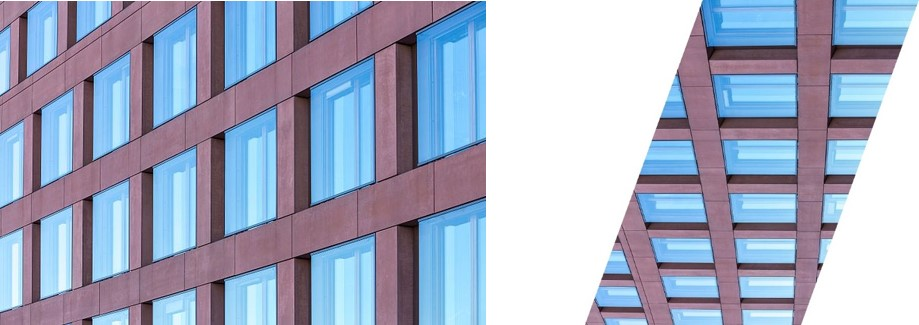
\includegraphics[height=1.5in]{twobuildings.jpg}
\end{image}

Not all transformations are matrix transformations.  Practice Problem \ref{prob:translation_does_not_work} offers a cautionary tale of what happens when we try to find a matrix for a transformation when such a matrix does not exist.
Luckily, many familiar transformations, including rotations, scalings, reflections, and shears, are matrix transformations. We will focus our attention on those.

Recall that by Observation \ref{obs:imagesOfijk} of \href{https://ximera.osu.edu/oerlinalg/LinearAlgebra/LTR-0005/main}{Matrix Transformations}, we can find a matrix for each transformation by examining what the transformation does to the standard basis vectors $\vec{i}$ and $\vec{j}$. 

\subsection*{Horizontal and Vertical Scaling} 

\begin{exploration}\label{init:vertstretch} Let us attempt to find a matrix $M$ for the transformation $T$ that stretches an image vertically by a factor of 2, as shown in the figure below.  

\begin{center}
		\begin{tikzpicture}[scale=2]
\node[inner sep=0pt, anchor=base] (gulls) at (6.25mm,0)
  {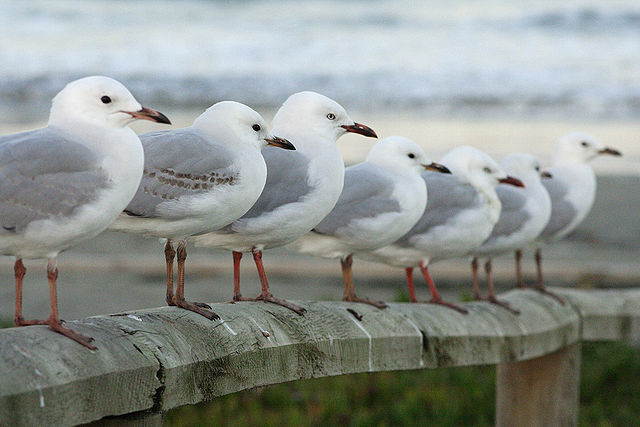
\includegraphics[width=25mm]{gulls.jpg}};
  \draw[<->] (-0.5,0)--(2,0);
  \draw[<->] (0,-0.5)--(0,2);
       \end{tikzpicture}
  \quad\quad
   \begin{tikzpicture}[scale=2]
 \node[inner sep=0pt, anchor=base]  (stretchedgulls) at (6.25mm,0)
  {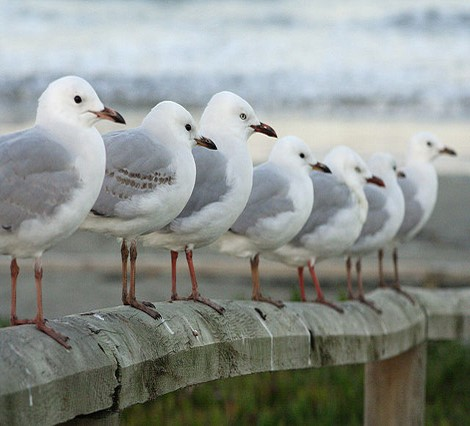
\includegraphics[width=25mm]{stretchedgulls.jpg}};
\draw[<->] (-0.5,0)--(2,0);
  \draw[<->] (0,-0.5)--(0,2);
    \end{tikzpicture}
    \end{center}

Consider what this transformation does to the standard unit vectors.  We observe that $T(\vec{i})=\vec{i}$ and $T(\vec{j})=2\vec{j}$. 

\begin{center}
\begin{tikzpicture}[scale=1.5]

  \draw[<->] (-0.5,0)--(2.5,0);
  \draw[<->] (0,-0.5)--(0,2.5);
   \draw[->,line width=1pt,red,-stealth](0,0)--(1,0);
   \node[red] at (0.5, -0.2)   (a) {$\vec{i}$};
    \draw[->,line width=1pt,blue,-stealth](0,0)--(0,1);
    \node[blue] at (-0.2, 0.5)   (b) {$\vec{j}$};
  \end{tikzpicture}
  \quad\quad
    \begin{tikzpicture}[scale=1.5]
\draw[<->] (-0.5,0)--(2.5,0);
  \draw[<->] (0,-0.5)--(0,2.5);
  \node[red] at (0.5, -0.2)   (a) {$T(\vec{i})$};
  \node[blue] at (-0.3, 1)   (b) {$T(\vec{j})$};
   \draw[->,line width=1pt,red,-stealth](0,0)--(1,0);
    \draw[->,line width=1pt,blue,-stealth](0,0)--(0,2);
    
 \end{tikzpicture}
 \end{center}
%\end{image}

 This allows us to construct a candidate for the transformation matrix $M$, by making the images of $\vec{i}$ and $\vec{j}$ the columns of $M$.  Thus, 
$$M=\begin{bmatrix}
1 & 0\\
0 & 2
\end{bmatrix}$$

We can now check to see what this matrix does to an arbitrary point $(a, b)$.  Treating this point as a vector $\begin{bmatrix}a\\b\end{bmatrix}$, we compute
$$M=\begin{bmatrix}
1 & 0\\
0 & 2
\end{bmatrix}\begin{bmatrix}a\\b\end{bmatrix}=\begin{bmatrix}a\\2b\end{bmatrix}$$
 Thus, this transformation takes point $(a, b)$ to point $(a, 2b)$.  So, the proposed transformation doubles all $y$-coordinates resulting in a vertical stretch by a factor of 2.
\end{exploration}






 In general, a vertical stretch (or compression) leaves $\vec{i}$ unchanged, and scales the vector $\vec{j}$ while preserving its vertical direction.  Thus, a vertical stretch (or compression) maps $\vec{i}$ to $\vec{i}$, and maps $\vec{j}$ to $k\vec{j}$ for some positive number $k$.  Similarly, a horizontal stretch (or compression) maps $\vec{i}$ to $k\vec{i}$, and maps $\vec{j}$ to $\vec{j}$.


\begin{formula}[Horizontal and Vertical Scaling] \label{form:horvertscaling}
  
 A matrix transformation induced by 
  \begin{equation} \label{vscale}
M_v=\begin{bmatrix}
1 & 0\\
0 & k
\end{bmatrix},
\end{equation}
where ($k>0$), scales objects in the plane vertically by a factor of $k$.

A matrix transformation induced by
  \begin{equation} \label{hscale}
M_h=\begin{bmatrix}
k & 0\\
0 & 1
\end{bmatrix},
\end{equation}
where ($k>0$), scales objects in the plane horizontally by a factor of $k$.
\end{formula}

In stating the above formula we stipulated that $k>0$.  If we were to allow $k$ to be zero, what would the resulting transformations accomplish?  In what way would the resulting matrices be fundamentally different from matrices $M_v$ and $M_h$?  What would happen if $k$ were allowed to be negative? (See Practice Problem \ref{prob:k0})

\subsection*{Horizontal and Vertical Shears}
A \dfn{horizontal shear} is a transformation that takes an arbitrary point $(a, b)$ and maps it to the point $(a+kb, b)$.  The effect of this transformation is that all points along a fixed horizontal line slide to the left or to the right by a fixed amount.  Note that the higher the point $(a, b)$ is above the $x$-axis, the greater is the magnitude of $kb$, resulting in a greater amount of horizontal slide.

%\begin{figure}[h]
%\begin{image}[4in]
\begin{center}
\begin{tikzpicture}[scale=0.8]

  \draw[<->] (-2,0)--(4,0);
   \draw[<->] (0,-2)--(0,4);
  \draw[dashed] (-2,-1)--(4,-1);
  \draw[dashed] (-2,1)--(4,1);
  \draw[dashed] (-2,2)--(4,2);
  \draw[dashed] (-2,3)--(4,3);
  
  
  \fill[] (0,-1) circle (0.1cm);
  \fill[] (1,-1) circle (0.1cm);
  \fill[] (2,-1) circle (0.1cm);
   
  \fill[red] (0,0) circle (0.1cm);
  \fill[red] (1,0) circle (0.1cm);
  \fill[red] (2,0) circle (0.1cm);
  
  \fill[blue] (0,1) circle (0.1cm);
  \fill[blue] (1,1) circle (0.1cm);
  \fill[blue] (2,1) circle (0.1cm);
  
  \fill[gray] (0,2) circle (0.1cm);
  \fill[gray] (1,2) circle (0.1cm);
  \fill[gray] (2,2) circle (0.1cm);
  
  \fill[orange] (0,3) circle (0.1cm);
  \fill[orange] (1,3) circle (0.1cm);
  \fill[orange] (2,3) circle (0.1cm);
  
   
  \end{tikzpicture}
   \quad\quad
\begin{tikzpicture}[scale=0.8]

\draw[<->] (-2,0)--(4,0);
  \draw[<->] (0,-2)--(0,4);
  \draw[dashed] (-2,-1)--(4,-1);
  \draw[dashed] (-2,1)--(4,1);
  \draw[dashed] (-2,2)--(4,2);
  \draw[dashed] (-2,3)--(4,3);
   
   \fill[] (0-0.5,-1) circle (0.1cm);
  \fill[] (1-0.5,-1) circle (0.1cm);
  \fill[] (2-0.5,-1) circle (0.1cm);
   
  \fill[red] (0,0) circle (0.1cm);
  \fill[red] (1,0) circle (0.1cm);
  \fill[red] (2,0) circle (0.1cm);
  
  \fill[blue] (0+0.5,1) circle (0.1cm);
  \fill[blue] (1+0.5,1) circle (0.1cm);
  \fill[blue] (2+0.5,1) circle (0.1cm);
  
  \fill[gray] (0+1,2) circle (0.1cm);
  \fill[gray] (2,2) circle (0.1cm);
  \fill[gray] (3,2) circle (0.1cm);
  
  \fill[orange] (1.5,3) circle (0.1cm);
  \fill[orange] (2.5,3) circle (0.1cm);
  \fill[orange] (3.5,3) circle (0.1cm);
 
 \end{tikzpicture}
%\end{image}
\end{center}

Adding a scalar multiple of the $y$ component to the $x$ component can be accomplished by matrix multiplication.  Observe that 
$$\begin{bmatrix}
1 & k\\
0 & 1
\end{bmatrix}\begin{bmatrix}a\\b\end{bmatrix}=\begin{bmatrix}a+kb\\b\end{bmatrix}$$

A \dfn{vertical shear} is a transformation that takes an arbitrary point $(a, b)$ and maps it to the point $(a, b+ka)$.  This too, can be accomplished by matrix multiplication.
$$\begin{bmatrix}
1 & 0\\
k & 1
\end{bmatrix}\begin{bmatrix}a\\b\end{bmatrix}=\begin{bmatrix}a\\b+ka\end{bmatrix}$$

\begin{formula}[Horizontal and Vertical Shears]\label{form:shears}
  
A matrix transformation induced by 
  \begin{equation} 
M_{hs}=\begin{bmatrix}
1 & k\\
0 & 1
\end{bmatrix}
\end{equation}
shears the plane horizontally.

A matrix transformation induced by
  \begin{equation} 
M_{vs}=\begin{bmatrix}
1 & 0\\
k & 1
\end{bmatrix}
\end{equation}
shears the plane vertically.
\end{formula}

\begin{example}\label{ex:vertshear1} Find the matrix $M_{vs}$ of a matrix transformation $T$ that {\it shears} the image of a seagull, as shown in the figure below. 

%\begin{figure}[h]
%\begin{image}[4in]
  \begin{center} 
		\begin{tikzpicture}[scale=2]
\node[inner sep=0pt, anchor=base] (gulls) at (6.25mm,0)
  {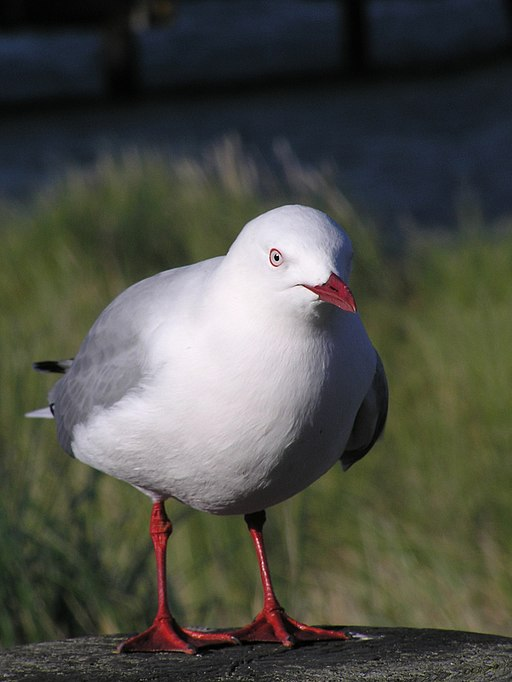
\includegraphics[width=25mm]{gull.jpg}};
  \draw[<->] (-0.5,0)--(2,0);
  \draw[<->] (0,-0.5)--(0,2);
       \end{tikzpicture}
  \quad\quad
\begin{tikzpicture}[scale=2]
 \node[inner sep=0pt, anchor=base]  (stretchedgulls) at (6.25mm,0)
  {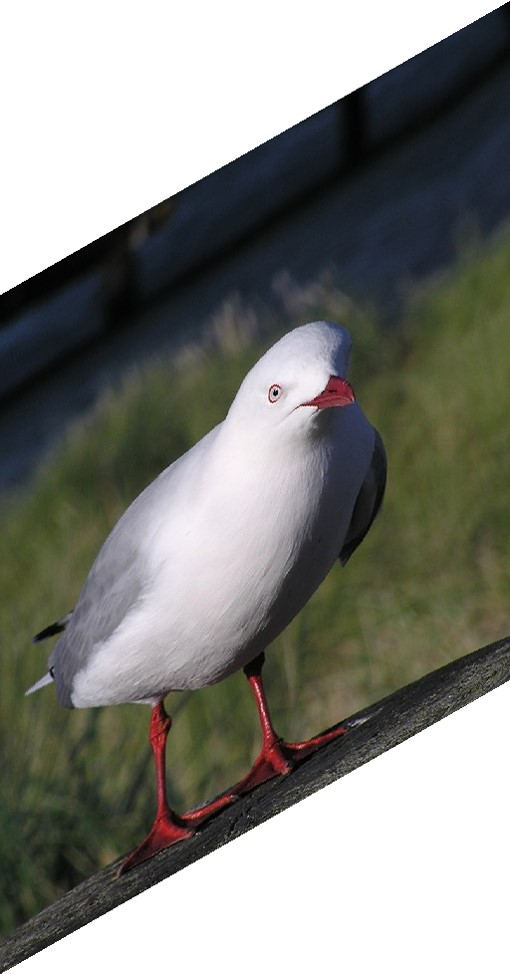
\includegraphics[width=25mm]{shearedgull.jpg}};
  
  \draw (0.5,0) arc (0:30:0.5);
  \node[] at (0.75, 0.2)   (a) {$30^{\circ}$};

\draw[<->] (-0.5,0)--(2,0);
  \draw[<->] (0,-0.5)--(0,2);
    
 \end{tikzpicture}
%\end{image}
\end{center}

\begin{explanation}
Consider what this transformation does to the standard unit vectors.

%\begin{figure}[h]

%\begin{image}[4in]
\begin{center}
\begin{tikzpicture}[scale=2]

  \draw[<->] (-0.5,0)--(1.5,0);
  \draw[<->] (0,-0.5)--(0,1.5);
   \draw[->,line width=1pt,red,-stealth](0,0)--(1,0);
    \draw[->,line width=1pt,blue,-stealth](0,0)--(0,1);
    \node[red] at (0.5, -0.1)   (a) {$\vec{i}$};
  \node[blue] at (-0.1, 0.5)   (b) {$\vec{j}$};
  \end{tikzpicture}
   \quad\quad
\begin{tikzpicture}[scale=2]

\draw[<->] (-0.5,0)--(1.5,0);
  \draw[<->] (0,-0.5)--(0,1.5);
  \fill[] (1,0.58)node[above]{$(1,\tan 30^{\circ})$} circle (0.03cm);   
   \draw[->,line width=1pt,red,-stealth](0,0)--(1,0.58);
    \draw[->,line width=1pt,blue,-stealth](0,0)--(0,1);
    \node[red] at (0.65, 0.15)   (a) {$T(\vec{i})$};
  \node[blue] at (-0.2, 0.5)   (b) {$T(\vec{j})$};
  \end{tikzpicture}
%  \end{image}
\end{center}

The tip of the vector $\vec{i}$ slides up a vertical line and its $x$-component remains the same.  Vector $\vec{j}$ stays fixed.  We observe that $T(\vec{i})=\begin{bmatrix}
1 \\
\tan 30^{\circ}
\end{bmatrix}=\begin{bmatrix}
1 \\
\sqrt{3}/3
\end{bmatrix}$ and $T(\vec{j})=\vec{j}$.  This allows us to construct $M_{vs}$, by making the images of $\vec{i}$ and $\vec{j}$ the columns of $M_{vs}$.  Thus, 
$$M_{vs}=\begin{bmatrix}
1 & 0\\
\sqrt{3}/3 & 1
\end{bmatrix}$$
\end{explanation}
\end{example}



\subsection*{Rotations about the Origin}
It turns out that rotations about the origin are also matrix transformations.  You will have an opportunity to revisit and prove this claim in Problem \ref{prob:linOfRotRef} of \href{https://ximera.osu.edu/oerlinalg/LinearAlgebra/SUPX-0060/main}{Additional Exercises}.

\begin{example}\label{ex: rotate45} Let $R_{45^{\circ}}:\RR^2\rightarrow\RR^2$ be a transformation that rotates $\RR^2$ countercolockwise about the origin by $45^{\circ}$.  Find a matrix that induces $R_{45^{\circ}}$.

%\begin{image}[4in]
 \begin{center}   
		\begin{tikzpicture}[scale=1.3]
\node[inner sep=0pt] (tower) at (0,0)
  {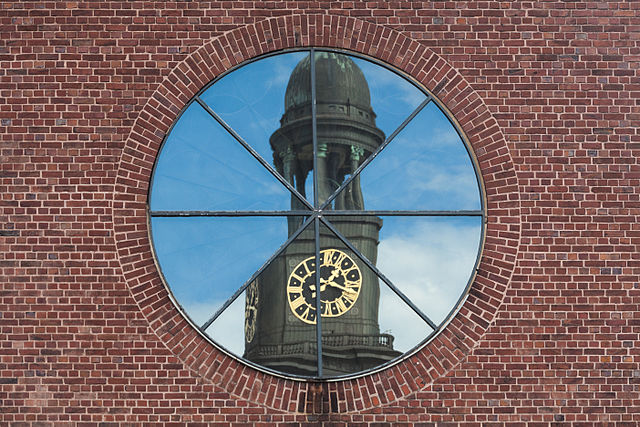
\includegraphics[width=45mm]{tower.jpg}};
  \draw[<->] (-2,0)--(2,0);
  \draw[<->] (0,-2)--(0,2);
       \end{tikzpicture}\quad
\begin{tikzpicture}[scale=1.3]
\node[inner sep=0pt] (tower) at (0,0)
  {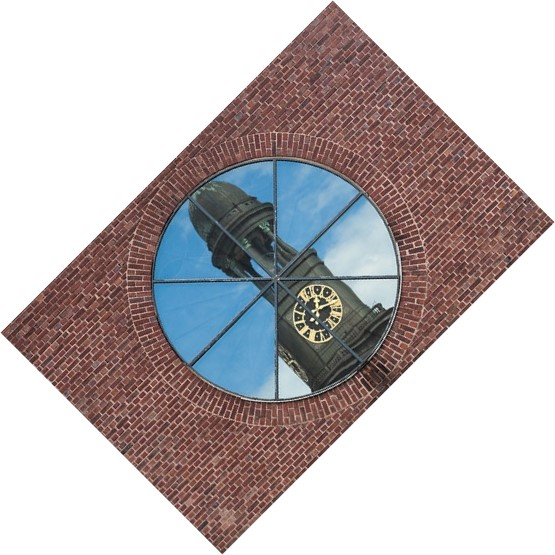
\includegraphics[width=50mm]{rotatedtower.jpg}};
  \draw[<->] (-2,0)--(2,0);
  \draw[<->] (0,-2)--(0,2);
       \end{tikzpicture}
%\end{image}
\end{center}

\begin{explanation}  Consider the action of $R_{\theta}$ on the standard unit vectors. 

%\begin{image}[4.5in]   
\begin{center}
\begin{tikzpicture}[scale=2.2]
    \node[red] at (0.5, -0.1)   (a) {$\vec{i}$};
    \node[blue] at (-0.1, 0.5)   (b) {$\vec{j}$};
  \draw[<->] (-0.5,0)--(1.5,0);
  \draw[<->] (0,-0.5)--(0,1.5);
   \draw[->,line width=1pt,red,-stealth](0,0)--(1,0);
    \draw[->,line width=1pt,blue,-stealth](0,0)--(0,1);
  \end{tikzpicture}
  \quad
  \begin{tikzpicture}[scale=2.2]
\node[red] at (0.3, 0.5)   (a) {$T(\vec{i})$};
    \node[blue] at (-0.5, 0.2)   (b) {$T(\vec{j})$};
     \node[] at (-0.7, 0.9)   (c) {$(-\sin 45^{\circ}, \cos 45^{\circ})$};
      \node[] at (0.7, 0.9)   (c) {$(\cos 45^{\circ}, \sin 45^{\circ})$};
  \draw[<->] (0,-0.5)--(0,1.5);
  \draw[<->] (-1,0)--(1,0);
  \fill[] (0.71,0.71) circle (0.03cm); 
  \fill[] (-0.71,0.71) circle (0.03cm); 
   \draw[->,line width=1pt,red,-stealth](0,0)--(0.71,0.71);
    \draw[->,line width=1pt,blue,-stealth](0,0)--(-0.71,0.71);
 \filldraw[blue, opacity=0.2](0,0)--(0.71,0.71)--(0.71,0)--cycle;
 \filldraw[orange, opacity=0.3](0,0)--(-0.71,0.71)--(0,0.71)--cycle;
  \draw (0.25,0) arc (0:45:0.25) ;
  \draw (0,0.25) arc (90:135:0.25) ;
  \node[] at (-0.15, 0.35)   (a) {$45^{\circ}$};
\node[] at (0.40, 0.15)   (b) {$45^{\circ}$};
 \end{tikzpicture}

\end{center}



We observe that $R_{\theta}(\vec{i})=\begin{bmatrix}
\cos 45^{\circ} \\
\sin 45^{\circ}
\end{bmatrix}=\begin{bmatrix}
\frac{\sqrt{2}}{2} \\
\frac{\sqrt{2}}{2}
\end{bmatrix}$ and $R_{\theta}(\vec{j})=\begin{bmatrix}
-\sin 45^{\circ} \\
\cos 45^{\circ}
\end{bmatrix}=\begin{bmatrix}
-\frac{\sqrt{2}}{2} \\
\frac{\sqrt{2}}{2}
\end{bmatrix}$.  This allows us to construct the matrix $M_{\theta}$, by making the images of $\vec{i}$ and $\vec{j}$ the columns of $M_{\theta}$.  Thus, 
$$M_{\theta}=\begin{bmatrix}
\frac{\sqrt{2}}{2} & -\frac{\sqrt{2}}{2}\\
\frac{\sqrt{2}}{2} & \frac{\sqrt{2}}{2}
\end{bmatrix}$$
\end{explanation}
\end{example}

In general, we find the rotation matrix by determining the images of vectors $\vec{i}$ and $\vec{j}$.

\begin{center}
\begin{tikzpicture}[scale=2.5]
  \draw[<->] (-0.5,0)--(1.5,0);
  \draw[<->] (0,-0.5)--(0,1.5);
  \node[red] at (0.5, -0.1)   (a) {$\vec{i}$};
    \node[blue] at (-0.1, 0.5)   (b) {$\vec{j}$};
   \draw[->,line width=1pt,red,-stealth](0,0)--(1,0);
    \draw[->,line width=1pt,blue,-stealth](0,0)--(0,1);
  \end{tikzpicture}
  \quad
\begin{tikzpicture}[scale=2.5]
\node[blue] at (-0.5, 0.5)   (a) {$R_{\theta}(\vec{j})$};
\node[red] at (0.4, 0.4)   (b) {$R_{\theta}(\vec{i})$};

\node[] at (0.9, 0.6)   (c) {$(\cos \theta,\sin \theta)$};
\node[] at (-0.5, 1)   (d) {$(-\sin \theta, \cos \theta)$};

\node[] at (-0.15, 0.55)   (a) {$\theta$};
\node[] at (0.55, 0.15)   (b) {$\theta$};
\draw[<->] (-1,0)--(1,0);
  \draw[<->] (0,-0.5)--(0,1.5);
  \fill[] (0.87,0.5) circle (0.03cm); 
  \fill[] (-0.5, 0.87) circle (0.03cm); 
   \draw[->,line width=1pt,red,-stealth](0,0)--(0.87,0.5);
    \draw[->,line width=1pt,blue,-stealth](0,0)--(-0.5, 0.87);
 \draw (0.5,0) arc (0:30:0.5) ;
  \draw (0,0.5) arc (90:120:0.5) ;
 \end{tikzpicture}
 \end{center}


\begin{formula}[Counterclockwise Rotation]\label{form:rotation}
    A matrix transformation induced by
    \begin{equation} \label{eq:rotation}
M_{\theta}=\begin{bmatrix}
\cos\theta & -\sin\theta\\
\sin\theta & \cos\theta
\end{bmatrix}
\end{equation}
rotates the plane counterclockwise through angle $\theta$ about the origin.
\end{formula}

\subsection*{Reflections about Lines of the Form $y=mx$}
When a point is reflected about a line, its image is located on the opposite side of the line and the same distance away from the line as the original point.  This is another example of a matrix transformation.  (We will prove that this is a matrix transformation in Problem \ref{prob:linOfRotRef} of \href{https://ximera.osu.edu/oerlinalg/LinearAlgebra/SUPX-0060/main}{Additional Exercises}.)

For example, the figure below shows the reflection of point $A$ about line $l$.  Note that the reflection lies on a line through $A$ perpendicular to $l$.

\begin{center}
\begin{tikzpicture}[scale=1.2]

   \draw[line width=1pt](-1,2)node[below, left]{$l$}--(1,-2);
  \draw[thin, dashed](-2,-1.5)--(2,0.5);
  
  \fill[red](1,0) circle (0.08)node[above]{$A$};
  \fill[](-0.6,-0.8) circle (0.08);
    \end{tikzpicture}
    \end{center}
 %   \end{image}
 
Our task is to find the matrix of a reflection of the plane about an arbitrary line through the origin.  
  

\begin{exploration}\label{init:reflectionxyaxes}
In this problem we will find the matrix for the reflection about the $x$ and $y$ axes.  You can easily do this on your own by finding the images of vectors $\vec{i}$ and $\vec{j}$.  
  
  We will start with the reflection about the $x$-axis.
  
  $$\vec{i}=\begin{bmatrix}1\\0\end{bmatrix}\quad\text{maps to}\quad\begin{bmatrix}\answer{1}\\\answer{0}\end{bmatrix}$$
  
  $$\vec{j}=\begin{bmatrix}0\\1\end{bmatrix}\quad\text{maps to}\quad\begin{bmatrix}\answer{0}\\\answer{-1}\end{bmatrix}$$
  
  So, the matrix that induces the reflection about the $x$-axis is
  $$\begin{bmatrix}\answer{1}&\answer{0}\\\answer{0}&\answer{-1}\end{bmatrix}$$
Next, we will consider the reflection about the $y$-axis.
$$\vec{i}=\begin{bmatrix}1\\0\end{bmatrix}\quad\text{maps to}\quad\begin{bmatrix}\answer{-1}\\\answer{0}\end{bmatrix}$$
  
  $$\vec{j}=\begin{bmatrix}0\\1\end{bmatrix}\quad\text{maps to}\quad\begin{bmatrix}\answer{0}\\\answer{1}\end{bmatrix}$$
  
  Thus, the matrix that induces the reflection about the $y$-axis is
  $$\begin{bmatrix}\answer{-1}&\answer{0}\\\answer{0}&\answer{1}\end{bmatrix}$$
  
  \end{exploration}
  
  Now we will turn our attention to transformations that reflect the plane about the line $y=mx$.  We will assume that $m\neq 0$.
  
  Consider the vector $\vec{i}$ and its reflection. 
%\begin{figure}[h]
%\begin{image}[2.2in]
\begin{center}
\begin{tikzpicture}[scale=1.2]

  \draw[<->] (-2,0)--(2,0);
  \draw[<->] (0,-2)--(0,2);

  \draw[line width=1pt](-1,2)node[below, left]{$y=mx$}--(1,-2);
  \draw[thin, dashed](-2,-1.5)node[below]{$y=-\frac{1}{m}x+\frac{1}{m}$}--(2,0.5);
  \node[red] at (0.5, 0.2)   (a) {$\vec{i}$};
  \node[] at (-0.5, -0.2)   (b) {$T(\vec{i})$};
  \draw[->,line width=1pt, -stealth, red](0,0)--(1,0);
  \draw[->,line width=1pt, -stealth](0,0)--(-0.6,-0.8);
  \draw[dashed] (0,0) circle (1);
 
  \end{tikzpicture}
  \end{center}
  %\end{image}

   
   
   
   Observe that the head of the image vector, $T(\vec{i})$, will lie on the line that passes through $(1,0)$ and is perpendicular to the line $y=mx$.  The equation of this line is given by
   
   \begin{equation}\label{eq:reflectionline} 
   y=-\frac{1}{m}x+\frac{1}{m}
   \end{equation}
   
 The head of $T(\vec{i})$ will also lie on the circle with equation
   $$x^2+y^2=1$$
   
   
   To find the image of $\vec{i}$ we need to determine where the line  $y=-\frac{1}{m}x+\frac{1}{m}$ intersects the circle.  Substitution gives us
   
   $$x^2+\left(-\frac{1}{m}x+\frac{1}{m}\right)^2=1$$
   After a little algebra we get
   $$\left(1+\frac{1}{m^2}\right)x^2-\left(\frac{2}{m^2}\right)x+\left(\frac{1}{m^2}-1\right)=0$$
   The quadratic formula yields 
   $$x=1\quad\text{and}\quad x=\frac{1-m^2}{m^2+1}$$
   
   The solution $x=1$ corresponds to the head of the vector $\vec{i}$.  So, the $x$-component of $T(\vec{i})$ is $x=\frac{1-m^2}{m^2+1}$.  We find the $y$-component of $T(\vec{i})$ by
   substituting $x=\frac{1-m^2}{m^2+1}$ into Equation \ref{eq:reflectionline}.
   $$ y=-\frac{1}{m}\left(\frac{1-m^2}{m^2+1}\right)+\frac{1}{m}=\frac{2m}{m^2+1}$$
   Thus, the image of $\vec{i}$ under this reflection is given by
   $$T(\vec{i})=\begin{bmatrix}\frac{1-m^2}{m^2+1}\\\frac{2m}{m^2+1}\end{bmatrix}$$
   
Next we need to find the image of $\vec{j}$. The head of $T(\vec{j})$ is located at one of the intersections of line $y=-\frac{1}{m}x+1$ and the circle $x^2+y^2=1$.  
   

% \begin{image}[2.2in]
\begin{center}
\begin{tikzpicture}[scale=1.2]

  \draw[<->] (-2,0)--(2,0);
  \draw[<->] (0,-2)--(0,2);
 
  \draw[line width=1pt](-1,2)--(1,-2)node[above, right]{$y=mx$};
  \draw[thin, dashed](-2,0)--(2,2)node[below,right]{$y=-\frac{1}{m}x+1$};
  \node[blue] at (0.15, 0.5)   (a) {$\vec{j}$};
  \draw[->,line width=1pt, -stealth, blue](0,0)--(0,1);
  \draw[->,line width=1pt, -stealth](0,0)--(-0.8,0.6)node[above, left]{$T(\vec{j})$};
  \draw[dashed] (0,0) circle (1);
  \end{tikzpicture}
  \end{center}
 % \end{image}


We leave it to the reader to verify that
\begin{equation}\label{eq:imageofj} T(\vec{j})=\begin{bmatrix}\frac{2m}{m^2+1}\\\frac{m^2-1}{m^2+1}\end{bmatrix}\end{equation}

This reflection is induced by the matrix 
$$M_{y=mx}=\begin{bmatrix}\frac{1-m^2}{m^2+1} & \frac{2m}{m^2+1}\\\frac{2m}{m^2+1} & \frac{m^2-1}{m^2+1}\end{bmatrix}=\frac{1}{1+m^2}\begin{bmatrix}
1-m^2 & 2m \\
2m & m^2-1
\end{bmatrix}$$

\begin{formula}[Reflection about the line $y=mx$]\label{form:reflection}
  
  A matrix transformation induced by
\begin{equation} \label{eq:reflectionymx}
M_{y=mx}=\frac{1}{1+m^2}\begin{bmatrix}
1-m^2 & 2m \\
2m & m^2-1
\end{bmatrix}
\end{equation}
reflects the plane about the line $y=mx$.
\end{formula}
Note that when $m=0$, expression (\ref{eq:reflectionymx}) is consistent with the reflection matrix you found in Exploration \ref{init:reflectionxyaxes}.

\begin{example}\label{ex:reflectedduck} Find matrix $M$ that reflects the image of the duck about the line $y=\frac{3}{5}x$.

%\begin{figure}[h]
%\begin{image}[4in]
\begin{center}
		\begin{tikzpicture}[scale=2]
\node[inner sep=0pt, anchor=base] (gulls) at (6.25mm,0)
  {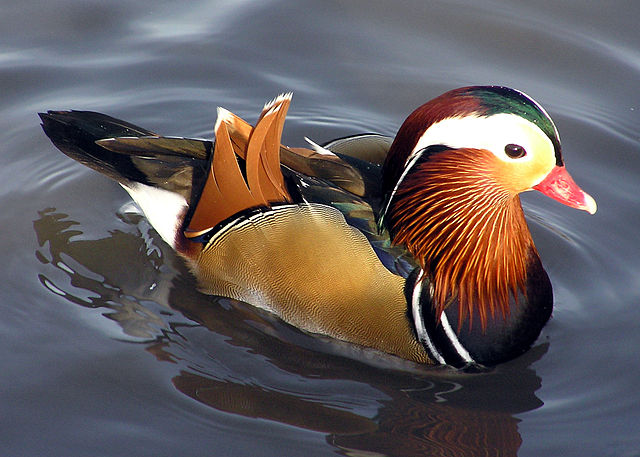
\includegraphics[width=25mm]{duck.jpg}};
  \draw[<->] (-0.5,0)--(2,0);
  \draw[<->] (0,-0.5)--(0,1.5);
  \draw[red,thick] (0,0)--(2,1.2);
  \node[red] at (1.5, 1.3)   (a) {$y=\frac{3}{5}x$};
       \end{tikzpicture}
   \quad
\begin{tikzpicture}[scale=2]
 \node[inner sep=0pt, anchor=base]  (stretchedgulls) at (6.875mm,-4.2mm)
  {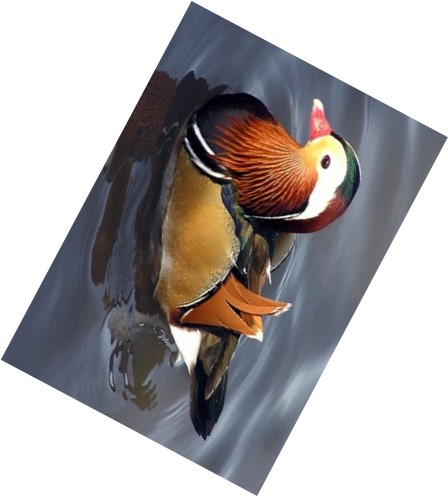
\includegraphics[width=27.5mm]{reflectedduck.jpg}};
  \node[red] at (1.5, 1.3)   (a) {$y=\frac{3}{5}x$};
\draw[red,thick] (0,0)--(2,1.2);
\draw[<->] (-0.5,0)--(2,0);
  \draw[<->] (0,-0.5)--(0,1.5);
    
 \end{tikzpicture}
 \end{center}
% \end{image}
% \caption{The original photo of the duck was reflected about he line $y=\frac{3}{5}x$.}
%  \label{fig:reflectedduck} 
%\end{figure}
\begin{explanation}
$$M=\frac{1}{1+9/25}\begin{bmatrix}1-9/25 & 6/5\\6/5 & 9/25 -1\end{bmatrix}=\frac{25}{34}\begin{bmatrix}16/25 & 6/5\\6/5 & -16/25\end{bmatrix}=\begin{bmatrix}8/17 & 15/17\\15/17 & -8/17\end{bmatrix}$$
\end{explanation}
\end{example}

Note that the eye of the duck in Example \ref{ex:reflectedduck} is located on the line $y=\frac{3}{5}x$.  The reflection leaves the eye fixed in place.  The eye is an example of a \dfn{fixed point}.  In Practice Problem \ref{prob:fixedpoint} you will be asked to show that every point along the line $y=\frac{3}{5}x$ is a fixed point.

\subsection*{Composition of Linear Transformations}

If a matrix transformation is followed by another matrix transformation, the resulting transformation can be represented as a product of the two matrices that induce the individual transformations.  Thus, if $T_1$ is induced by $M_1$ and $T_2$ is induced by $M_2$, then $T=T_2\circ T_1$ is induced by $M=M_2M_1$.

\begin{center}
\begin{tikzpicture}
\node{
\begin{tikzcd}
\RR^2\rar{T_1}\arrow[black, bend right]{rr}[black,swap]{T}  & \RR^2 \rar{T_2}  & \RR^2
\end{tikzcd}
};
\end{tikzpicture}
\end{center}

Remember that matrix multiplication is not commutative, so the order in which the matrices are multiplied is of utmost importance.

Consider the following example which incorporates a reflection as well as a rotation of vectors.

\begin{example}\label{exa:rotationreflection}
\begin{enumerate}
    \item Find the matrix of the linear transformation which is obtained by first rotating all vectors counterclockwise by an angle of $\pi /6$ and then reflecting across the $x$-axis.
    \item Multiply the vector $\vec{v}=\begin{bmatrix}
    1/2 \\ \sqrt{3}/2 \end{bmatrix}$ by the matrix you found in part (a) to illustrate how the transformation works.
\end{enumerate}


\begin{explanation}
\begin{enumerate}
    \item 

Using Formula \ref{form:rotation}, the matrix of the transformation which
involves rotating through an angle of $\pi /6$ is
\begin{equation*}
M_1 =
\begin{bmatrix}
\cos \left( \pi /6\right) & -\sin \left( \pi /6\right) \\
\sin \left( \pi /6\right) & \cos \left( \pi /6\right)
\end{bmatrix}
 =
\begin{bmatrix}
\frac{1}{2}\sqrt{3} & -\frac{1}{2} \\
\frac{1}{2} & \frac{1}{2}\sqrt{3}
\end{bmatrix}
\end{equation*}

As we learned in Exploration \ref{init:reflectionxyaxes}, the matrix for the transformation which reflects all vectors about the $x$-axis is $M_2 = \begin{bmatrix}1 & 0 \\ 0 & -1 \end{bmatrix}$.

Therefore, the matrix of the linear transformation which first rotates
through $\pi /6$ and then reflects through the $x$-axis is given by
\begin{equation*}
M = M_2 M_1 = 
\begin{bmatrix}1 & 0 \\ 0 & -1 \end{bmatrix} \begin{bmatrix}
\frac{1}{2}\sqrt{3} & -\frac{1}{2} \\
\frac{1}{2} & \frac{1}{2}\sqrt{3}
\end{bmatrix} = \begin{bmatrix}
\frac{1}{2}\sqrt{3} & \frac{1}{2} \\
-\frac{1}{2} & -\frac{1}{2}\sqrt{3}
\end{bmatrix}
\end{equation*}

\item From unit circle trigonometry, we know that $\vec{v}$ makes a $\pi/3$ angle with the $x$-axis.  If we rotate $\vec{v}$ counterclockwise by $\pi /6$, it will point straight up.  

\begin{center}
\begin{tikzpicture}[scale=2]
  \draw[<->] (-0.5,0)--(1,0);
  \draw[<->] (0,-0.5)--(0,1.5);
\draw[line width=1pt, blue, stealth-](0.5,1.73/2)--(0,0);
\draw[line width=1pt, red, -stealth](0,0)--(0,1);
\fill[blue] (0.4,0.3)node[right]{$\pi/3$};
\fill[red] (0.2,0.7)node[above]{$\pi/6$};
\draw[blue] (0.4,0) arc (0:60:0.4) ;
\draw[red] (0.25,1.73/4) arc (60:90:0.5) ;
\node[blue] at (0.9, 1.75/2)   (b) {$(\frac{1}{2},\frac{\sqrt{3}}{2})$}; 
 \end{tikzpicture}
\end{center}


Following the rotation with reflection across the $x$-axis will make it point straight down.  Sure enough, 
$$M\vec{v} = \begin{bmatrix}
\frac{1}{2}\sqrt{3} & -\frac{1}{2} \\
-\frac{1}{2} & -\frac{1}{2}\sqrt{3}
\end{bmatrix} \begin{bmatrix}
    1/2 \\ \sqrt{3}/2 \end{bmatrix} = \begin{bmatrix}
    0 \\ -1 \end{bmatrix}.$$
\end{enumerate}
\end{explanation} 
\end{example}

\begin{exploration}\label{exp:matrixComp}
You can use the GeoGebra interactive below to decompose a matrix into a product of two matrices corresponding to the basic transformations we discussed above: scalings, rotations, shears and reflections.

Consider the matrix $M=\begin{bmatrix} 1 & 0\\-1 & -1\end{bmatrix}$.  This matrix induces a transformation that can be broken into two parts: (1) a reflection followed by (2) a shear.  Find matrices $M_1$ and $M_2$ that induce the reflection and the shear respectively.  Verify that the product of the two matrices is equal to $M$ (be careful about the order of the product!).
$$M=M_2M_1=\begin{bmatrix}\answer{1}&\answer{0}\\\answer{-1}&\answer{1}\end{bmatrix}\begin{bmatrix}\answer{1}&\answer{0}\\\answer{0}&\answer{-1}\end{bmatrix}$$
\begin{center}
\geogebra{d6jyt85s}{950}{500}
\end{center}
Let  $M=\begin{bmatrix}-1&0\\0&-1\end{bmatrix}$.  Use the GeoGebra interactive above to visually examine the transformation induced by $M$.  The composition of which transformations is equivalent to the transformation induced by $M$? 
\begin{multipleChoice}  
\choice{Rotation by 180 degrees.}  
\choice{Reflection about the $x$-axis, followed by a reflection about the $y$-axis.}
\choice{Reflection about the $y$-axis, followed by a reflection about the $x$-axis.}  
\choice[correct]{All of the above.}
\end{multipleChoice} 

Let $M=\begin{bmatrix}0&1\\-1&0\end{bmatrix}$.  Use the GeoGebra interactive above to visually examine the transformation induced by $M$.
The composition of which transformations is equivalent to the transformation induced by $M$? 
\begin{multipleChoice}  
\choice[correct]{Reflection about the $x$-axis, followed by a reflection about the line $y=-x$.}
\choice{Reflection about the $y$-axis, followed by a reflection about the $x$-axis.}  
\choice{All of the above.}
\choice{None of the above.}
\end{multipleChoice} 
\end{exploration}


\begin{example}\label{init:reflectioncomp}  In this problem we will consider compositions of two reflections and use geometry to illustrate non-commutativity of matrix multiplication.  
Let $$T_{y=-2x}:\RR^2\rightarrow \RR^2$$ be a reflection about the line $y=-2x$.  Let $$T_{y=x}:\RR^2\rightarrow \RR^2$$ be a reflection about the line $y=x$. We will denote the standard matrices for these transformations by $M_{y=-2x}$ and $M_{y=x}$, and
use geometry to demonstrate that $M_{y=x}M_{y=-2x}\neq M_{y=-2x}M_{y=x}$.  
 
 To do this, consider transformations $T_1=T_{y=x}\circ T_{y=-2x}$ and $T_2=T_{y=-2x}\circ T_{y=x}$.  Transformation $T_1$ is induced by $M_{y=x}M_{y=-2x}$, and $T_2$ is induced by $M_{y=-2x}M_{y=x}$.

The figure on the left illustrates the action of $T_1$ on a single point $A$.  First, $A$ is reflected about the line $y=-2x$, then $A$ is reflected about the line $y=x$.   

The figure on the right shows the action of $T_2$ on the same point $A$.  The point is first reflected about the line $y=x$, followed by a reflection about the line $y=-2x$.  The final images of point $A$ under $T_1$ and $T_2$ are clearly different.

\begin{center}
\begin{tikzpicture}[scale=.3]
\draw[thin,gray!40] (-8,-8) grid (8,8);
  \draw[<->] (-8,0)--(8,0);
  \draw[<->] (0,-8)--(0,8);
  \draw[line width=1pt,blue](-8,-8)--(8,8)node[below=4mm]{$y=x$} ;
  \draw[line width=1pt,red](-4,8)--(4,-8)node[above=2mm, right=1mm]{$y=-2x$};
 
  \draw[gray, dashed] (-5,5)--(-1,7);
  \draw[gray, dashed] (-1,7)--(7,-1);
  \fill[] (-5,5)node[above=2mm, left=1mm]{$A$} circle (0.2cm);
  \fill[] (-1,7)node[above=3mm]{} circle (0.2cm);
  \fill[] (7,-1)node[below=2mm]{$T_1(A)$} circle (0.3cm);
  \end{tikzpicture}
  \quad\quad
\begin{tikzpicture}[scale=.3]
 
\draw[thin,gray!40] (-8,-8) grid (8,8);
  \draw[<->] (-8,0)--(8,0);
  \draw[<->] (0,-8)--(0,8);
\draw[gray, dashed] (-5,5)--(5,-5);
  \draw[gray, dashed] (5,-5)--(1,-7);
  \fill[] (-5,5)node[above=2mm, left=1mm]{$A$} circle (0.2cm);
  \fill[] (5,-5)node[above=3mm]{} circle (0.2cm);
  \fill[] (1,-7)node[left=2mm]{$T_2(A)$} circle (0.3cm);
  the transformation induced by
  \draw[line width=1pt,blue](-8,-8)--(8,8)node[below=4mm]{$y=x$} ;
  \draw[line width=1pt,red](-4,8)--(4,-8)node[above=2mm, right=1mm]{$y=-2x$} ;
 \end{tikzpicture}
%\end{image}
\end{center}

Since $T_1\neq T_2$, we conclude that $M_{y=x}M_{y=-2x}\neq M_{y=-2x}M_{y=x}$.

\end{example}

\begin{example}\label{ex:rotationscommute}
Some pairs of matrices do commute.  For example, geometry makes it is easy to see that two rotation matrices commute.
\end{example}

\section*{Practice Problems}
\begin{problem}\label{prob:k0}
Consider matrices $M_v$ and $M_h$ in (\ref{vscale}) and (\ref{hscale}).  
\begin{enumerate}
\item
If we were to allow $k$ to be zero, what would the resulting transformations accomplish?  
\item If $k=0$, in what way would the resulting matrices be fundamentally different from matrices $M_v$ and $M_h$ $(k\neq 0)$?  
\item Do $M_v$ and $M_h$ $(k\neq 0)$ have inverses?  What about $M_v$ and $M_h$ $(k= 0)$?  
\item What would happen if we allowed $k$ to be negative?
\end{enumerate}
\end{problem}

\begin{problem}\label{prob:matrixlintrans} Find a matrix $M$ that would double the length of a photo horizontally, and triple the height of the photo.
$$M=\begin{bmatrix}\answer{2} & \answer{0}\\\answer{0} & \answer{3}\end{bmatrix}$$
\end{problem}

\begin{problem}\label{prob:shearedsheep}
(Sheared Sheep) Find a matrix that induces the transformation shown in the figure. 
%\begin{image}[4in]
   \begin{center}
		\begin{tikzpicture}[scale=2]
\node[inner sep=0pt, anchor=base] (gulls) at (8.75mm,0)
  {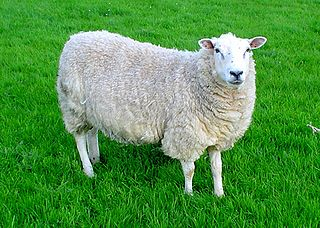
\includegraphics[width=35mm]{sheep.jpg}};
  \draw[<->] (-0.25,0)--(2,0);
  \draw[<->] (0,-0.25)--(0,1.8);
       \end{tikzpicture}
  \quad
\begin{tikzpicture}[scale=2]
 
 \node[inner sep=0pt, anchor=base]  (stretchedgulls) at (12.35mm,0)
  {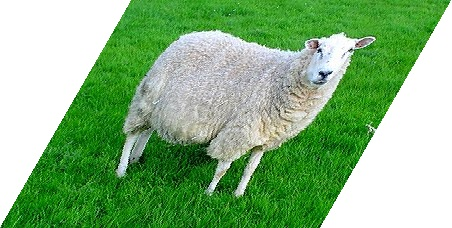
\includegraphics[width=49.4mm]{shearedsheep.jpg}};
  \node[] at (2.4, 0.25)   (a) {$60^{\circ}$};
 \draw (22.3mm,0) arc (0:60:0.5) ;

\draw[<->] (-0.25,0)--(3,0);
  \draw[<->] (0,-0.25)--(0,1.8);
    
 \end{tikzpicture}
 \end{center}
%\end{image}

\end{problem}

\begin{problem}\label{prob:translation_does_not_work}

Suppose a 1 by 1 photo of a chipmunk was shifted as shown in the figure. 
%\begin{image}[4.2in]  
\begin{center}
		\begin{tikzpicture}[scale=2]
\node[inner sep=0pt, anchor=base] (gulls) at (6.25mm,0)
  {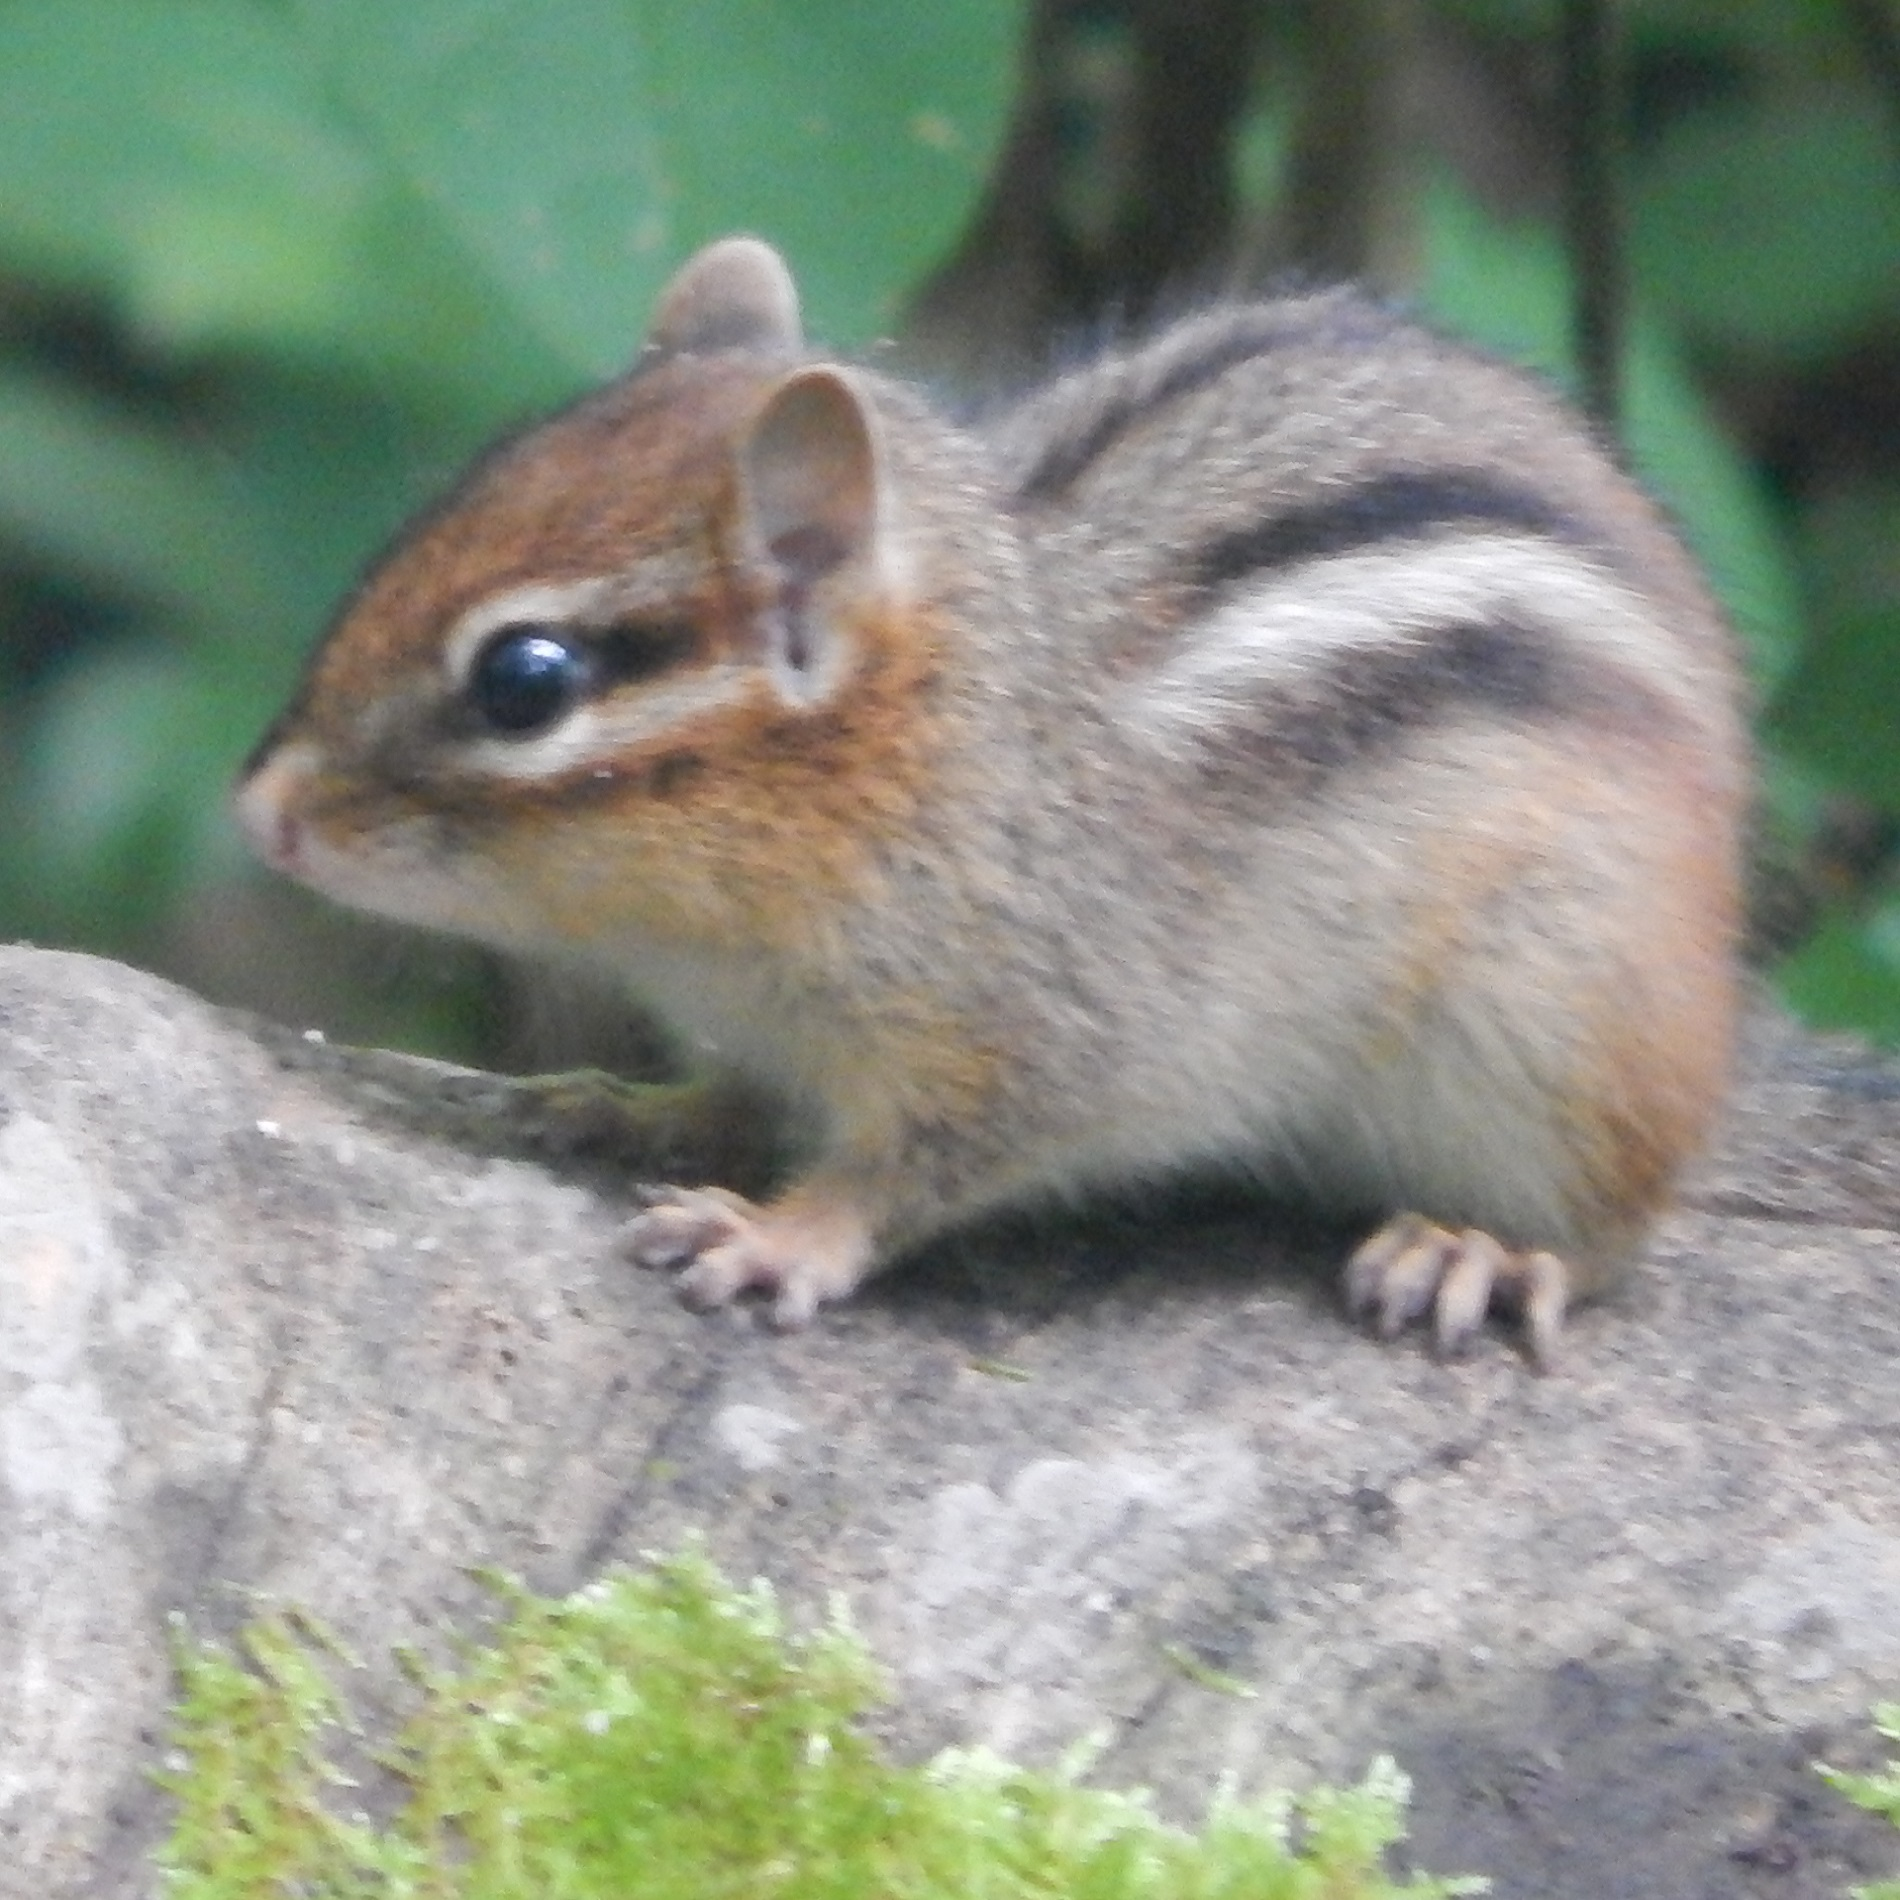
\includegraphics[width=25mm]{chipmunk.jpg}};
  \draw[<->] (-0.5,0)--(2,0);
  \draw[<->] (0,-0.5)--(0,2);
  \draw[->,red, line width=1mm, -stealth] (0mm,0mm)--(12.5mm,0mm)node[below right]{$(1, 0)$};
  \draw[->,blue, line width=1mm, -stealth] (0mm,0mm)--(0mm,12.5mm)node[above left]{$(0, 1)$};
       \end{tikzpicture}
  \quad\quad
   \begin{tikzpicture}[scale=2]
 \node[inner sep=0pt, anchor=base]  (stretchedgulls) at (11.25mm,5mm)
  {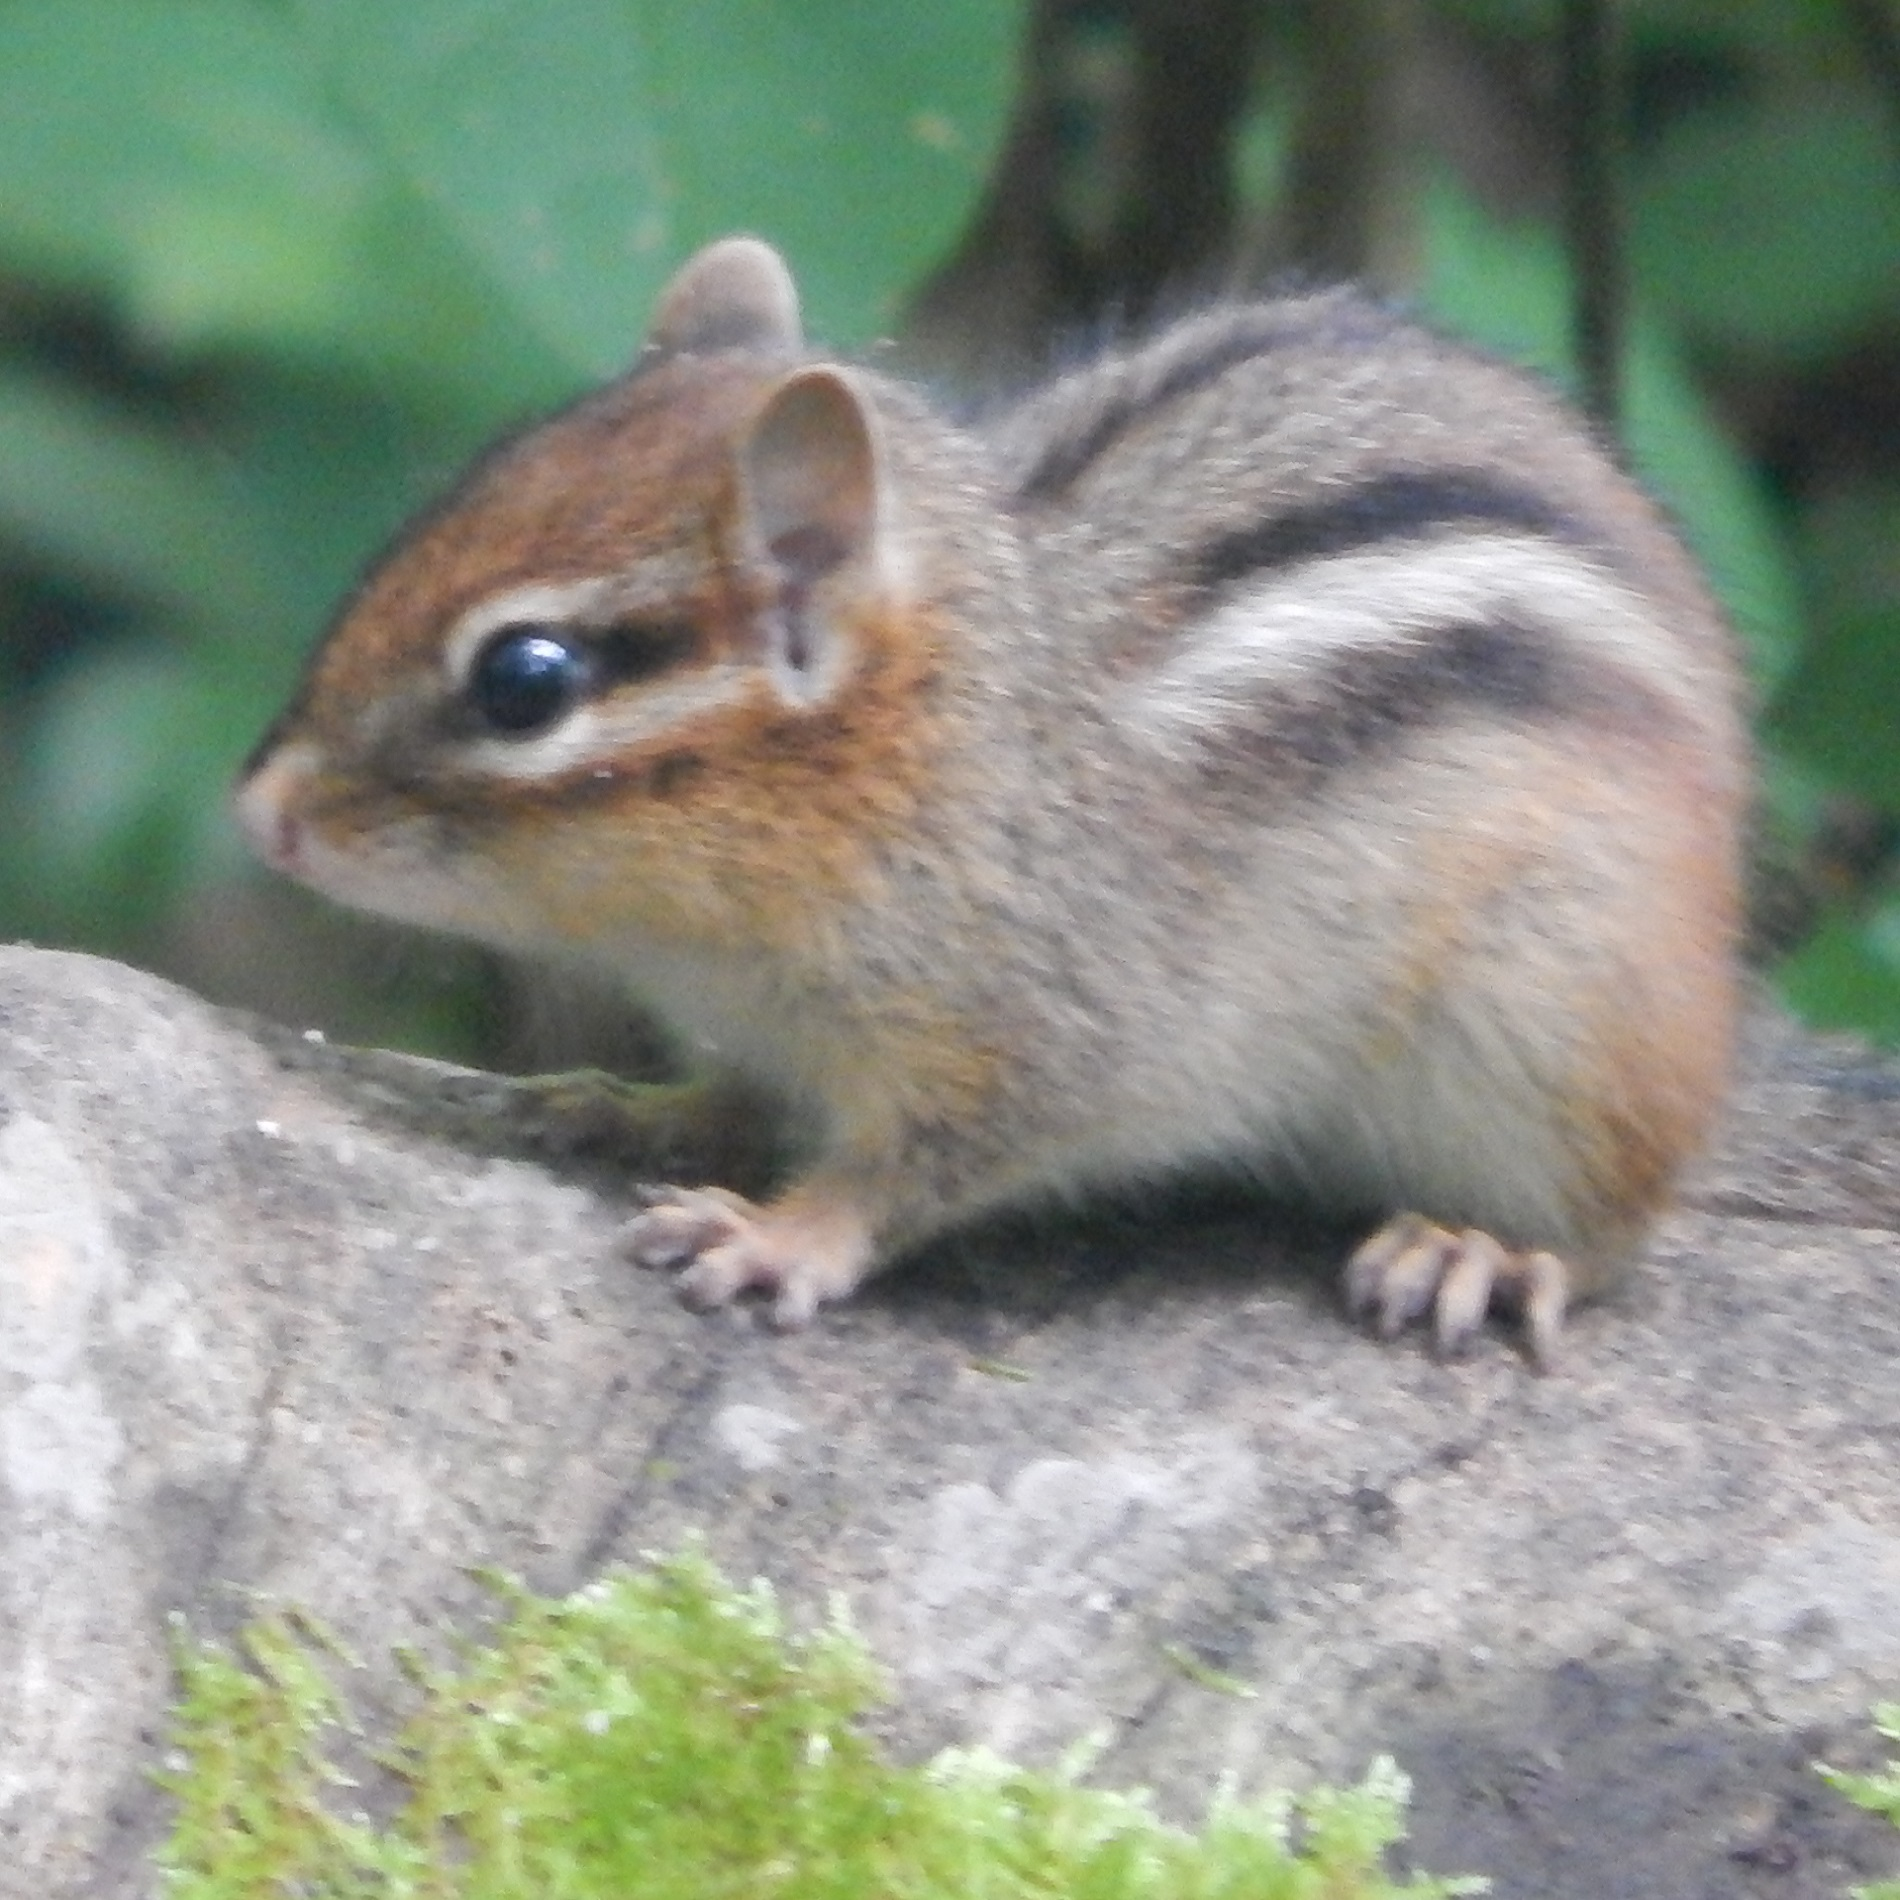
\includegraphics[width=25mm]{chipmunk.jpg}};
\draw[<->] (-0.5,0)--(2,0);
  \draw[<->] (0,-0.5)--(0,2);
  \draw[->,red, line width=1mm, -stealth] (0mm,0mm)--(17.5mm,5mm)node[below right]{$(1.4, 0.4)$};
  \draw[->,blue, line width=1mm, -stealth] (0mm,0mm)--(5mm,17.5mm)node[above right]{$(0.4, 1.4)$};
    \end{tikzpicture}
    \end{center}
%\end{image}

Suppose we tried to construct a standard matrix $M$ for this transformation by making the images of $\vec{i}$ and $\vec{j}$ the columns of $M$.  We would obtain
$$M=\begin{bmatrix}1.4 & 0.4\\0.4 & 1.4\end{bmatrix}$$
Does this matrix describe the transformation?  If so, prove it.  If not, explain why not.
\end{problem}

\begin{problem}\label{prob:translationtrans}
A transformation $T:\RR^2\rightarrow \RR^2$ that shifts all points in the plane horizontally or vertically by a fixed amount is called a \dfn{translation}.  Is $T$ a matrix transformation?  Prove your claim.
\begin{hint}
    Use Problem \ref{prb:6.4}
\end{hint}
\end{problem}

\begin{problem}\label{prob:reflectreflect} A reflection about the line $y=mx$ followed by another reflection about the same line, returns all points to their original position.  Prove this using matrix multiplication.
\begin{hint}
    Find the product of $M_{y=mx}M_{y=mx}$.
\end{hint}
\end{problem}

\begin{problem} \label{prob:imageofj}
Verify Equation (\ref{eq:imageofj}).
\end{problem}

\begin{problem}\label{prob:fixedpoint}
Prove that every point along the line $y=\frac{3}{5}x$ in Example \ref{ex:reflectedduck} is a fixed point.
\end{problem}

\begin{problem}\label{prob:reflectedduck}
The figure below shows a sequence of two matrix transformations that accomplishes a reflection about the line $y=\frac{3}{5}x$.  The first transformation is a reflection of the plane about the $x$-axis.  The second transformation is a rotation of the plane about the origin.  Find matrices that induce the two transformations and verify that their product (in the correct order) is the reflection matrix of Example \ref{ex:reflectedduck}.
%\begin{figure}[h]
\begin{center}
     
		\begin{tikzpicture}[scale=2]
\node[inner sep=0pt, anchor=base] (gulls) at (6.25mm,0)
  {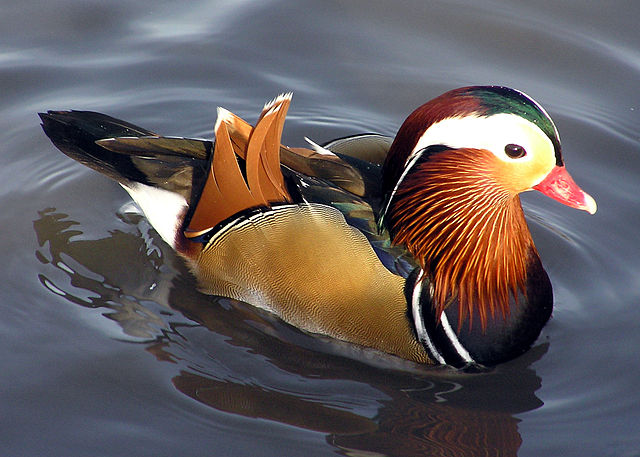
\includegraphics[width=25mm]{duck.jpg}};
  \draw[<->] (-0.5,0)--(2,0);
  \draw[<->] (0,-0.5)--(0,1.5);
  \draw[red,thick] (0,0)--(2,1.2);
  \node[red] at (1.5, 1.3)   (a) {$y=\frac{3}{5}x$};
       \end{tikzpicture}
\end{center}  
    
 \begin{center}      
		\begin{tikzpicture}[scale=2]
\node[inner sep=0pt, anchor=base] (gulls) at (6.25mm,-8.9mm)
  {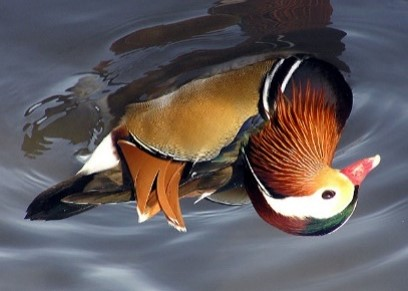
\includegraphics[width=25mm]{upsidedownduck.jpg}};
  \draw[<->] (-0.5,0)--(2,0);
  \draw[<->] (0,-1.5)--(0,1.5);
  \draw[red,thick] (0,0)--(2,1.2);
  \node[red] at (1.5, 1.3)   (a) {$y=\frac{3}{5}x$};
  \draw[dashed] (0,0)--(0.8,1.5)node[above=2mm, left=1mm]{};
       \end{tikzpicture}
 \end{center}  
    
 \begin{center}
\begin{tikzpicture}[scale=2]
 \node[inner sep=0pt, anchor=base]  (stretchedgulls) at (6.875mm,-4.2mm)
  {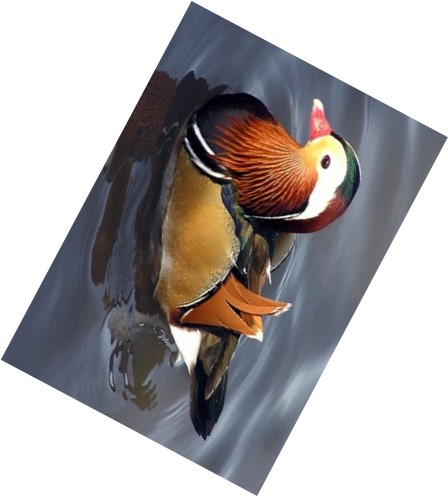
\includegraphics[width=27.5mm]{reflectedduck.jpg}};
  
  
\draw[red,thick] (0,0)--(2,1.2);
\node[red] at (1.5, 1.3)   (a) {$y=\frac{3}{5}x$};
\draw[<->] (-0.5,0)--(2,0);
  \draw[<->] (0,-0.5)--(0,1.5);
   \draw[dashed] (0,0)--(0.8,1.5)node[above=2mm, left=1mm]{}; 
 \end{tikzpicture}
\end{center}
 \end{problem}

\section*{Example Source}
Example \ref{exa:rotationreflection}  was adapted from Example 5.27  of Ken Kuttler's \href{https://open.umn.edu/opentextbooks/textbooks/a-first-course-in-linear-algebra-2017}{\it A First Course in Linear Algebra}. (CC-BY)

Ken Kuttler, {\it  A First Course in Linear Algebra}, Lyryx 2017, Open Edition, p. 290. 


\section*{Photo Credits}
The following images are courtesy of \href{https://commons.wikimedia.org/wiki/Main_Page}
{Wikimedia Commons}

Adrian Pingstone, \dfn{A male Mandarin Duck at Slimbridge Wildfowl and Wetlands Centre, Gloucestershire, England.} Public Domain

Ansgar Koreng, \dfn{Facade of ARD-Hauptstadtstudio in Berlin-Mitte.} CC-BY 4.0

Christoph Braun, \dfn{Reflection of St. Michaelis Church in a window of St. Ansgar in Hamburg, Germany.} Public Domain.

Daniel Gammert, \dfn{Red-billed Gulls Chroicocephalus novaehollandiae scopulinus. Brighton Beach, New Zealand.} Public Domain

 I, Tony Wills, \dfn{Red billed gull in Wellington Harbour, Wellington, New Zealand.}  CC-BY

Jackhynes, \dfn{Lleyn sheep taken with a Sony Digital Camera at 3.2 megapixels in Devon, UK.} Public Domain

Erik Davis, \dfn{Chipmunk.} CC-BY




\end{document} 